\documentclass{simcenterdocumentation}
\usepackage{amsmath,amssymb}
\usepackage{mathtools}
\usepackage{biblatex}

% To compile this file, run "latex/pdflatex TInF-documentation", then "biber TInF-documentation"
% (or "bibtex TInF-documentation", if the output from latex asks for that instead),
% and then "latex/pdflatex TInF-documentation" (without the quotes in each case).

% Double spacing, if you want it.  Do not use for the final copy. Can also specify
% draft as a document class option. This will generate double spacing and placeholders
% for title page and header images
%% \def\dsp{\def\baselinestretch{2.0}\large\normalsize}
%% \dsp

\usepackage{listings}
\usepackage{color}
\usepackage{float}
\usepackage{multirow}
\usepackage{graphicx}
\usepackage{subcaption}

\definecolor{dkgreen}{rgb}{0,0.6,0}
\definecolor{gray}{rgb}{0.5,0.5,0.5}
\definecolor{mauve}{rgb}{0.58,0,0.82}
\definecolor{lightgrey}{rgb}{0.95,0.95,0.95}
\definecolor{darkgrey}{rgb}{0.50,0.50,0.50}

\lstset{
  frame=shadowbox, 
  language=C,
  aboveskip=3mm,
  belowskip=3mm,
  showstringspaces=false,
  columns=flexible,
  basicstyle={\small\ttfamily},
  numbers=none,
  numberstyle=\tiny\color{gray},
  keywordstyle=\color{blue},
  commentstyle=\color{dkgreen},
  stringstyle=\color{mauve},
  breaklines=true,
  breakatwhitespace=true,
  tabsize=3,
  rulesepcolor=\color{darkgrey},
  backgroundcolor=\color{lightgrey}
}

\graphicspath{%
              {figs},%
	      {images/},%
	      {theory},%
	      {theory/figs}%
	     }

%%%%%%%%%%%%%%%%%%%%%%%%%%%%%%%%%%%%%%%%%%%%%%%%%%%%%%%%%%%%%%%%%%%%%%%
%
% gloabal layout settings
%
%%%%%%%%%%%%%%%%%%%%%%%%%%%%%%%%%%%%%%%%%%%%%%%%%%%%%%%%%%%%%%%%%%%%%%%

%
% paragraph layout
%
% \parindent	0pt
% \parskip	3pt plus2pt minus1pt
%
% border width of fbox
%
\fboxsep	10pt
\fboxrule	1pt
%
% placement of floats
%
\def\topfraction{0.95}
\def\bottomfraction{0.95}
\def\textfraction{0.05}

%%\setcounter{topnumber}{1}
%%\setcounter{bottomnumber}{1}
%
% debug messages
%
%%\hfuzz 1pt

%%%%%%%%%%%%%%%%%%%%%%%%%%%%%%%%%%%%%%%%%%%%%%%%%%%%%%%%%%%%%%%%%%%%%%%
%
% gloabal abbreviations
%
%%%%%%%%%%%%%%%%%%%%%%%%%%%%%%%%%%%%%%%%%%%%%%%%%%%%%%%%%%%%%%%%%%%%%%%

%
% where to find global definitions
%
\def\TeXDIR	{./TeX/}

%
% load glocal abbreviations file
%
% \usepackage{times,mathptm}
% \usepackage{\TeXDIR PSshort}
%\include{\TeXDIR kurz}

%
% layout style definitions
%
\def\DS{\displaystyle}
\def\TS{\textstyle}
\def\SS{\scriptstyle}

%%%%%%%%%%%%%%%%%%%%%%%%%%%%%%%%%%%%%%%%%%%%%%%%%%%%%%%%%%%%%%%%%%%%%%%
%
% definition of new environments
%
%%%%%%%%%%%%%%%%%%%%%%%%%%%%%%%%%%%%%%%%%%%%%%%%%%%%%%%%%%%%%%%%%%%%%%%

% \newcounter{cremark}
% \def\theremark{\arabic{cremark}}
\newcounter{cremark}[section]
\def\theremark{\thesection.\arabic{cremark}}

\newcounter{ctable}
\newenvironment{mybox}{%
                         \localeqn
			 \setcounter{ctable}{\value{table}}%
			 \refstepcounter{ctable}%
		         \def\theequation{\roman{equation}}%
		         % \def\theequation{\arabic{ctable}-\roman{equation}}%
			 \begin{minipage}[c]{0.95\hsize}%
			}%
                        {\par\end{minipage}%
			 \globaleqn\medskip}  
                        % {\hfill$\bullet$\par\medskip}  
\newenvironment{rem}{%
                         \refstepcounter{cremark}%
                         %\localeqn
		         %\def\theequation{\alph{equation}}%
			 \par
                         \penalty-1000
                         \medskip
                         \noindent
                         {\textbf{Remark~\theremark:}}%
                         % \penalty 10000
			 \leavevmode
			 \textsl\bgroup
			}%
                        {\egroup\par
			 %\globaleqn
			 \medskip}  
                        % {\hfill$\bullet$\par\medskip}  
\newcounter{saveequation}
\def\localeqn{\setcounter{saveequation}{\value{equation}}%
              \setcounter{equation}{0}%
	      \let\savetheqn\theequation}
\def\globaleqn{\setcounter{equation}{\value{saveequation}}%
               \let\theequation\savetheeqn}

%%%%%%%%%%%%%%%%%%%%%%%%%%%%%%%%%%%%%%%%%%%%%%%%%%%%%%%%%%%%%%%%%%%%%%%
%
% local abbreviations
%
%%%%%%%%%%%%%%%%%%%%%%%%%%%%%%%%%%%%%%%%%%%%%%%%%%%%%%%%%%%%%%%%%%%%%%%

\def\vectorform#1{\ensuremath{\left\{#1\right\}}}
\def\matrixform#1{\ensuremath{\left[#1\right]}}

\long\def\putinvector#1{\vectorform{\begin{array}{c}#1\end{array}}}
\long\def\putinmatrix#1{\matrixform{\begin{array}{ccc}#1\end{array}}}

\newcommand{\trace}{\mathop{\mathrm{tr}}}
\newcommand{\sign}{\mathop{\mathrm{sign}}}
\newcommand{\vol}{\mathop{\mathrm{vol}}}
\newcommand{\dev}{\mathop{\mathrm{dev}}}
\newcommand{\norm}[1]{\mathop{\left\Vert#1\right\Vert}}

\def\mathBox#1{\fbox{$\displaystyle #1$}}

\def\R{\mathbb{R}}
\def\N{\mathbb{N}}

%
% number spaces
%
\def\R		{\mathbb{R}}
\def\N		{\mathbb{N}}
\def\Rplus	{\R^+}
\def\Nplus	{\N^+}
\def\Roplus	{\R_0^+}
\def\Noplus	{\N_0^+}

%
% differential operations:
%
% ... total derivative
\newcommand{\diff}[2]{\frac{d #1}{d #2}}
%
% ... second order total derivative
\newcommand{\ddiff}[2]{\frac{d^2 #1}{d #2^2}}
%
% ... mixed second order total derivative
\def\mddiff#1#2#3{\frac{d^2 #1}{d #2\,d #3}}
%
% ... partial derivative
\newcommand{\pdiff}[2]{\frac{\partial #1}{\partial #2}}
%
% ... second order partial derivative
\newcommand{\pddiff}[2]{\frac{\partial^2 #1}{\partial #2^2}}
\newcommand{\ppdiff}[3]{\frac{\partial^2 #1}{\partial #2\otimes\partial #3}}
%
% ... mixed second order partial derivative
\def\mppdiff#1#2#3{\frac{\partial^2 #1}{\partial #2\,\partial #3}}

%
% text in formulas
%
\def\AND	{\hbox{and}}
\def\OR		{\hbox{or}}
\def\WITH	{\hbox{with}}

%
% tensor operators
%
\def\tr		{\mathop{\mathrm{tr}}}
\def\dev	{\mathop{\mathrm{dev}}}
\def\DEV	{\mathop{\mathrm{DEV}}}
\def\INV	{^{(-1)}}
\def\inv	{^{-1}}
\def\sqr	{^{2}}
\def\qub	{^{3}}
\def\Lie	{\mathcal{L}_v}

%\newcommand{\vectr}[1]{\mathbf{#1}}
\newcommand{\vectr}[1]{{\hbox{\boldmath$#1$}}}
\newcommand{\tensor}[1]{{\hbox{\boldmath$#1$}}}

\newcommand{\Div}{\mathop{\mathrm{Div}}}
\newcommand{\Grad}{\mathop{\mathrm{Grad}}}
\newcommand{\diver}{\mathop{\mathrm{div}}}
\newcommand{\grad}{\mathop{\mathrm{grad}}}
\newcommand{\deter}{\mathop{\mathrm{det}}}

%
% standard symbols
%

%
% special tensors (4th-order)
%
\def\I		{\mathbb{I}}
\def\IC		{\I_\vectr{C}}
\def\ICinv	{\I_{\Cinv}}
\def\Ib		{\I_\vectr{b}}
\def\IMi	{\I_{\stackrel{1}{\vectr{M}}}}
\def\IMii	{\I_{\stackrel{2}{\vectr{M}}}}
\def\IMiii	{\I_{\stackrel{3}{\vectr{M}}}}
\def\IMal	{\I_{\stackrel{\alpha}{\vectr{M}}}}
\def\IMbe	{\I_{\stackrel{\beta}{\vectr{M}}}}
\def\Imi	{\I_{\stackrel{1}{\vectr{m}}}}
\def\Imii	{\I_{\stackrel{2}{\vectr{m}}}}
\def\Imiii	{\I_{\stackrel{3}{\vectr{m}}}}
\def\Imal	{\I_{\stackrel{\alpha}{\vectr{m}}}}
\def\Imbe	{\I_{\stackrel{\beta}{\vectr{m}}}}

\def\IDEV	{\I^{\textrm{dev}}}
\def\Idev	{\left( \I-{\TS\frac{1}{3}}\,\Bone\otimes\Bone \right)}

%
% functions
%
\def\norm#1{\|#1\|}
\def\inpd#1{{<}#1{>}}




\bibliography{references}

\begin{document}
% Declarations for Front Matter
% Software title followed by optional second line
\title{TInF\\ \Large Turbulence Inflow Tool}
% Use superscripts to indicate author affiliations
\author{Jiawei Wan$^{1}$, Peter Mackenzie-Helnwein$^2$}
\institutions{$^1$University of Notre Dame \\$^2$University of Washington}
\softwarename{Turbulence Inflow Tool}
\softwareversion{1.0.2}

%%% DON'T MESS WITH THESE SETTINGS %%%%%%%%%%%%%%%%%%%%%%%%%%%%%%%%
\hypersetup{pageanchor=false}
\maketitle
\copyrightpage
\acknowledgments

\hypersetup{pageanchor=true}
\begin{frontmatter}

\pagestyle{plain}
{
  \renewcommand{\thispagestyle}[1]{}
  \tableofcontents
  \clearpage
  \listoffigures
  %\clearpage
  %\listoftables
}

\end{frontmatter}
\pagestyle{somewhatsimple}
%%%%%%%%%%%%%%%%%%%%%%%%%%%%%%%%%%%%%%%%%%%%%%%%%%%%%%%%%%%%%%%%%%%
% Create separate tex files for each chapter and provide them as inputs

\chapter{Tool Audience}
\section{Brief overview of some functionality available in \texttt{simcenterdocumentation.cls}}
You can access the software name, \getsoftwarename{}, like this
\texttt{\textbackslash getsoftwarename\{\}} after it has been input in
the preamble using \texttt{\textbackslash softwarename}. You can also
get the \insertsurveylink{link} to the feedback survey and place it in
the text using \texttt{\textbackslash insertsurveylink\{text\_for\_link\}}.

\vspace{0.25cm}
Code snippets with syntax highlighting can also be inserted:

\begin{python}[caption=Python script for analyzing the portal frame model with uncertain parameters]
  import numpy as np
  import os
  import shutil
  import subprocess
  from pyDOE import *
  from scipy.stats.distributions import norm  
#Setting number of samples
nSamples = 1000

#Creating latin hyper cube designs
design = lhs(2, samples=nSamples)

#Sampling Young's Modulus and Mass
ESamples = norm(loc=4227, scale=500.0).ppf(design[:,0])
mSamples = norm(loc=5.18, scale=1.0).ppf(design[:,1])
\end{python}

At present, this is only defined for \texttt{Python}, but can be easily extended in the class
for other languages. This in \textbf{no way} indicates any preference for a particular coding language
and should not be interpreted as a preference for \texttt{Python}.


\section{Faceplate Marginalia}

Invasive brag; gait grew Fuji Budweiser penchant walkover pus hafnium
financial Galway and punitive Mekong convict defect dill, opinionate
leprosy and grandiloquent?  Compulsory Rosa Olin
Jackson\cite{waveshaping} and pediatric Jan.  Serviceman, endow buoy
apparatus.

Forbearance.  Bois; blocky crucifixion September.\footnote{Davidson
witting and grammatic.  Hoofmark and Avogadro ionosphere.  Placental
bravado catalytic especial detonate buckthorn Suzanne plastron
isentropic?  Glory characteristic.  Denature?  Pigeonhole sportsman
grin historic stockpile.  Doctrinaire marginalia and art.  Sony
tomography.  Aviv censor seventh, conjugal.  Faceplate emittance
borough airline.  Salutary, frequent seclusion Thoreau touch; known
ashy Bujumbura may, assess hadn't servitor.  Wash doff, algorithm.}

\subsection{Promenade Exeter}

Inertia breakup Brookline.  Hebrew, prexy, and Balfour.  Salaam
applaud, puff teakettle.

\begin{quote}
Ugh servant Eulerian knowledge Prexy Lyman zig wiggly.  Promenade
adduce.  Yugoslavia piccolo Exeter.  Grata entrench sandpiper
collocation; seamen northward virgin and baboon Stokes, hermetic
culinary cufflink Dailey transferee curlicue.  Camille, Whittaker
harness shatter.  Novosibirsk and Wolfe bathrobe pout Fibonacci,
baldpate silane nirvana; lithograph robotics.  Krakow, downpour
effeminate Volstead?
\end{quote}

Davidson witting and grammatic.  Hoofmark and Avogadro ionosphere.
Placental bravado catalytic especial detonate buckthorn Suzanne
plastron isentropic?  Glory characteristic.  Denature?  Pigeonhole
sportsman grin historic stockpile.  Doctrinaire marginalia and art.
Sony tomography.  Aviv censor seventh, conjugal.  Faceplate emittance
borough airline.  Salutary.  Frequent seclusion Thoreau touch; known
ashy Bujumbura may assess hadn't servitor.  Wash, Doff, and Algorithm.


Davidson witting and grammatic.  Hoofmark and Avogadro ionosphere.
Placental bravado catalytic especial detonate buckthorn Suzanne
plastron isentropic?  Glory characteristic.  Denature?  Pigeonhole
sportsman grin historic stockpile. Doctrinaire marginalia and art.
Sony tomography.  Aviv censor seventh, conjugal.  Faceplate emittance
borough airline.  Salutary.  Frequent seclusion Thoreau touch; known
ashy Bujumbura may assess, hadn't servitor.  Wash, Doff, Algorithm.

\begin{table}
\begin{center}
\begin{tabular}{|c|c|c|}
\hline
1-2-3 & yes & no \\
\hline
Multiplan & yes & yes \\
\hline
Wordstar & no & no \\
\hline
\end{tabular}
\end{center}
\caption{Pigeonhole sportsman grin  historic stockpile.}
\end{table}
Davidson witting and grammatic.  Hoofmark and Avogadro ionosphere.
Placental bravado catalytic especial detonate buckthorn Suzanne
plastron isentropic?  Glory characteristic.  Denature?  Pigeonhole
sportsman grin historic stockpile. Doctrinaire marginalia and art.
Sony tomography.

\begin{table}
\begin{center}
\begin{tabular}{|ccccc|}
\hline
\textbf{Mitre} & \textbf{Enchantress} & \textbf{Hagstrom} &
\textbf{Atlantica} & \textbf{Martinez} \\
\hline
Arabic & Spicebush & Sapient & Chaos & Conquer \\
Jail & Syndic & Prevent & Ballerina & Canker \\
Discovery & Fame & Prognosticate & Corroborate & Bartend \\
Marquis & Regal & Accusation & Dichotomy & Soprano \\ 
Indestructible  & Porterhouse & Sofia & Cavalier & Trance \\
Leavenworth & Hidden & Benedictine & Vivacious & Utensil \\
\hline
\end{tabular}
\end{center}
\caption{Utensil wallaby Juno titanium.}
\end{table}

Aviv censor seventh, conjugal.  Faceplate emittance borough airline.
Salutary.  Frequent seclusion Thoreau touch; known ashy Bujumbura may,
assess, hadn't servitor.  Wash\cite{cmusic}, Doff, and Algorithm.

\begin{figure}
\[ \begin{picture}(90,50)
  \put(0,0){\circle*{5}}
  \put(0,0){\vector(1,1){31.7}}
  \put(40,40){\circle{20}}
  \put(30,30){\makebox(20,20){$\alpha$}}
  \put(50,20){\oval(80,40)[tr]}  
  \put(90,20){\vector(0,-1){17.5}}
  \put(90,0){\circle*{5}}
\end{picture}
 \]
\caption{Davidson witting and grammatic.  Hoofmark and Avogadro ionosphere.  
Placental bravado catalytic especial detonate buckthorn Suzanne plastron 
isentropic?  Glory characteristic.  Denature?  Pigeonhole sportsman grin.}
\end{figure}

Davidson witting and grammatic.  Hoofmark and Avogadro ionosphere.
Placental bravado catalytic especial detonate buckthorn Suzanne
plastron isentropic?  Glory characteristic.  Denature?  Pigeonhole
sportsman grin historic stockpile. Doctrinaire marginalia and art.
Sony tomography.  Aviv censor seventh, conjugal.  Faceplate emittance
borough airline.\cite{fm} Salutary.  Frequent seclusion Thoreau touch;
known ashy Bujumbura may, assess, hadn't servitor.  Wash, Doff, and
Algorithm.

\begin{itemize}
\item Davidson witting and grammatic.  Jukes foundry mesh sting speak,
Gillespie, Birmingham Bentley.  Hedgehog, swollen McGuire; gnat.
Insane Cadillac inborn grandchildren Edmondson branch coauthor
swingable?  Lap Kenney Gainesville infiltrate.  Leap and dump?
Spoilage bluegrass.  Diesel aboard Donaldson affectionate cod?
Vermiculite pemmican labour Greenberg derriere Hindu.  Stickle ferrule
savage jugging spidery and animism.
\item Hoofmark and Avogadro ionosphere.  
\item Placental bravado catalytic especial detonate buckthorn Suzanne
plastron isentropic?
\item Glory characteristic.  Denature?  Pigeonhole sportsman grin
historic stockpile.
\item Doctrinaire marginalia and art.  Sony tomography.  
\item Aviv censor seventh, conjugal.
\item Faceplate emittance borough airline.  
\item Salutary.  Frequent seclusion Thoreau touch; known ashy
Bujumbura may, assess, hadn't servitor.  Wash, Doff, and Algorithm.
\end{itemize}

Davidson witting and grammatic.  Hoofmark and Avogadro ionosphere.
Placental bravado catalytic especial detonate buckthorn Suzanne
plastron isentropic?  Glory characteristic.  Denature?  Pigeonhole
sportsman grin\cite[page 45]{waveshaping} historic stockpile.
Doctrinaire marginalia and art. Sony tomography.  Aviv censor seventh,
conjugal. Faceplate emittance borough airline.  Salutary.  Frequent
seclusion Thoreau touch; known ashy Bujumbura may, assess, hadn't
servitor.  Wash, Doff, and Algorithm.


\chapter{Introduction}
\section{Pigeonhole Buckthorn}

Davidson witting and grammatic.  Hoofmark and Avogadro ionosphere.
Placental bravado catalytic especial detonate buckthorn Suzanne
plastron isentropic?  Glory characteristic.  Denature?  Pigeonhole
sportsman grin historic stockpile. Doctrinaire marginalia and art.
Sony tomography.

\begin{figure}\centering
\parbox{.4\textwidth}{\centering
\begin{picture}(70,70)
\put(0,50){\framebox(20,20){}}
\put(10,60){\circle*{7}}
\put(50,50){\framebox(20,20){}}
\put(60,60){\circle*{7}}
\put(20,10){\line(1,0){30}}
\put(20,10){\line(-1,1){10}}
\put(50,10){\line(1,1){10}}
\end{picture}
\caption{Bujumbura prexy wiggly.}}
\hfill
\parbox{.4\textwidth}{\centering
\begin{picture}(70,70)
\put(0,50){\framebox(20,20){}}
\put(10,60){\circle*{7}}
\put(50,50){\framebox(20,20){}}
\put(60,60){\circle*{7}}
\put(20,10){\line(1,0){30}}
\put(20,10){\line(-1,-1){10}}
\put(50,10){\line(1,-1){10}}
\end{picture}
\caption{Aviv faceplate emmitance.}}
\end{figure}

Aviv censor seventh, conjugal.  Faceplate emittance borough airline.
Salutary.  Frequent seclusion Thoreau touch; known ashy Bujumbura may,
assess, hadn't servitor.  Wash, Doff, or Algorithm.

Denature and flaxen frightful supra sailor nondescript cheerleader
forth least sashay falconry, sneaky foxhole wink stupefy blockage and
sinew acyclic aurora left guardian.  Raffish daytime; fought ran and
fallible penning.

\section{Pinwheel Thresh}

Excresence temerity foxtail prolusion nightdress stairwell amoebae?
Pawnshop, inquisitor cornet credulous pediatric?  Conjoin.  Future
earthmen.  Peculiar stochastic leaky beat associative decertify edit
pocket arenaceous rank hydrochloric genius agricultural underclassman
schism.  Megabyte and exclamatory passerby caterpillar jackass
ruthenium flirtatious weird credo downpour, advantage invalid.

\section{Laryngeal Gallon Mission}

Conformance and pave.  Industrial compline dunk transept edifice
downstairs.  Sextillion.  Canvas?  Lyricism webbing insurgent
anthracnose treat familiar.  Apocalyptic quasar; ephemerides
circumstantial.

Peridotite giblet knot.  Navigable aver whee sheath bedraggle twill
era scourge insert.  Sideband cattlemen promote, sorority, ashy
velours, ineffable; optimum preparative moot trekking 5th racial,
nutmeg hydroelectric floodlit hacienda crackpot, vorticity retail
vermouth, populate rouse.  Ceremony?  Fungoid.


\chapter{Installation Instructions}
\label{sec:TInF-installation}

\section{Installing the Turbulence Inflow Tool}

Download the installation package for your operation system from (a single line)
\begin{verbatim}
https://www.designsafe-ci.org/data/browser/public/designsafe.storage.community/
            /SimCenter/Software/TurbulantInflowTool
\end{verbatim}
 SimCenter is providing packages for Windows~8/10 (64 bit version only) and MacOS.  
The installer will place the executable on your system.  On Windows systems, a shortcut will be added to your start menu.
On MacOS, the application is placed in your Applications folder.
\bigskip

For Linux systems, you will need to clone the source from 
\begin{verbatim}
https://github.com/NHERI-SimCenter/TurbulenceInflowTool
\end{verbatim}
and compile it yourself performing the following steps:
\begin{quote}
\begin{verbatim}
$ git clone https://github.com/NHERI-SimCenter/TurbulenceInflowTool
$ git clone https://github.com/NHERI-SimCenter/SimCenterCommon
$ cd TurbulenceInflowTool
$ qmake TurbulenceInflowTool.pro
$ make
$ sudo make install
\end{verbatim}
\end{quote}

\section{Compiling the Source Code in OpenFOAM}

Download the source code of the turbulent velocity boundary conditions from
\begin{verbatim}
https://github.com/NHERI-SimCenter/TurbulenceInflowTool/tree/master/openFOAM_code
\end{verbatim}

\noindent  The source code files are contained in a directory named \textcolor{blue}{inflowTurbulence}. Note that the code is provided for OpenFOAM version 6 and 7, and is slightly different in this two versions. Please choose the correct package to download according the version of OpenFOAM you have installed on your computer.

Create a project directory named \textcolor{blue}{run} within the \textcolor{blue}{\$HOME/OpenFOAM} directory named \textless{USER}\textgreater{-6} (e.g. Jack-6 for user Jack and OpenFOAM version 6) by typing the following script in a terminal prompt:

\begin{quote}
\begin{verbatim}
$ mkdir -p $FOAM_RUN
\end{verbatim}
\end{quote}

Copy or move the \textcolor{blue}{inflowTurbulence} directory which has been downloaded earlier and all the files in it to the \textcolor{blue}{\$HOME/OpenFOAM} directory. Go the relocated \textcolor{blue}{inflowTurbulence} directory by typing:

\begin{quote}
\begin{verbatim}
$ cd $FOAM_RUN/inflowTurbulence
\end{verbatim}
\end{quote}

Compile the codes in the \textcolor{blue}{inflowTurbulence} directory by typing the following in the terminal prompt:

\begin{quote}
\begin{verbatim}
$ wmake
\end{verbatim}
\end{quote}

After the compilation is successfully complete, a library file named \textcolor{blue}{libturbulentInflow.so} will be generated in the directory \textcolor{blue}{\$FOAM\_USER\_LIBBIN}.


\chapter{Usage}
\label{sec:TInF-usage}

The workflow for adding parameters for various kinds of turbulence inflow models to your 
OpenFOAM model is as follows.

\begin{description}
\item[Step~1: Source Selection] Start the Turbulence Inflow Tool (TInF) and on the opening screen select the Source Tab (Figure~\ref{fig:TInF01}, item~1).  Use the locate button (Figure~\ref{fig:TInF01}, item~3) to navigate to your OpenFOAM input tree.  
\begin{figure}[htb]
	\begin{center}
		\vspace*{-1.0\baselineskip}
		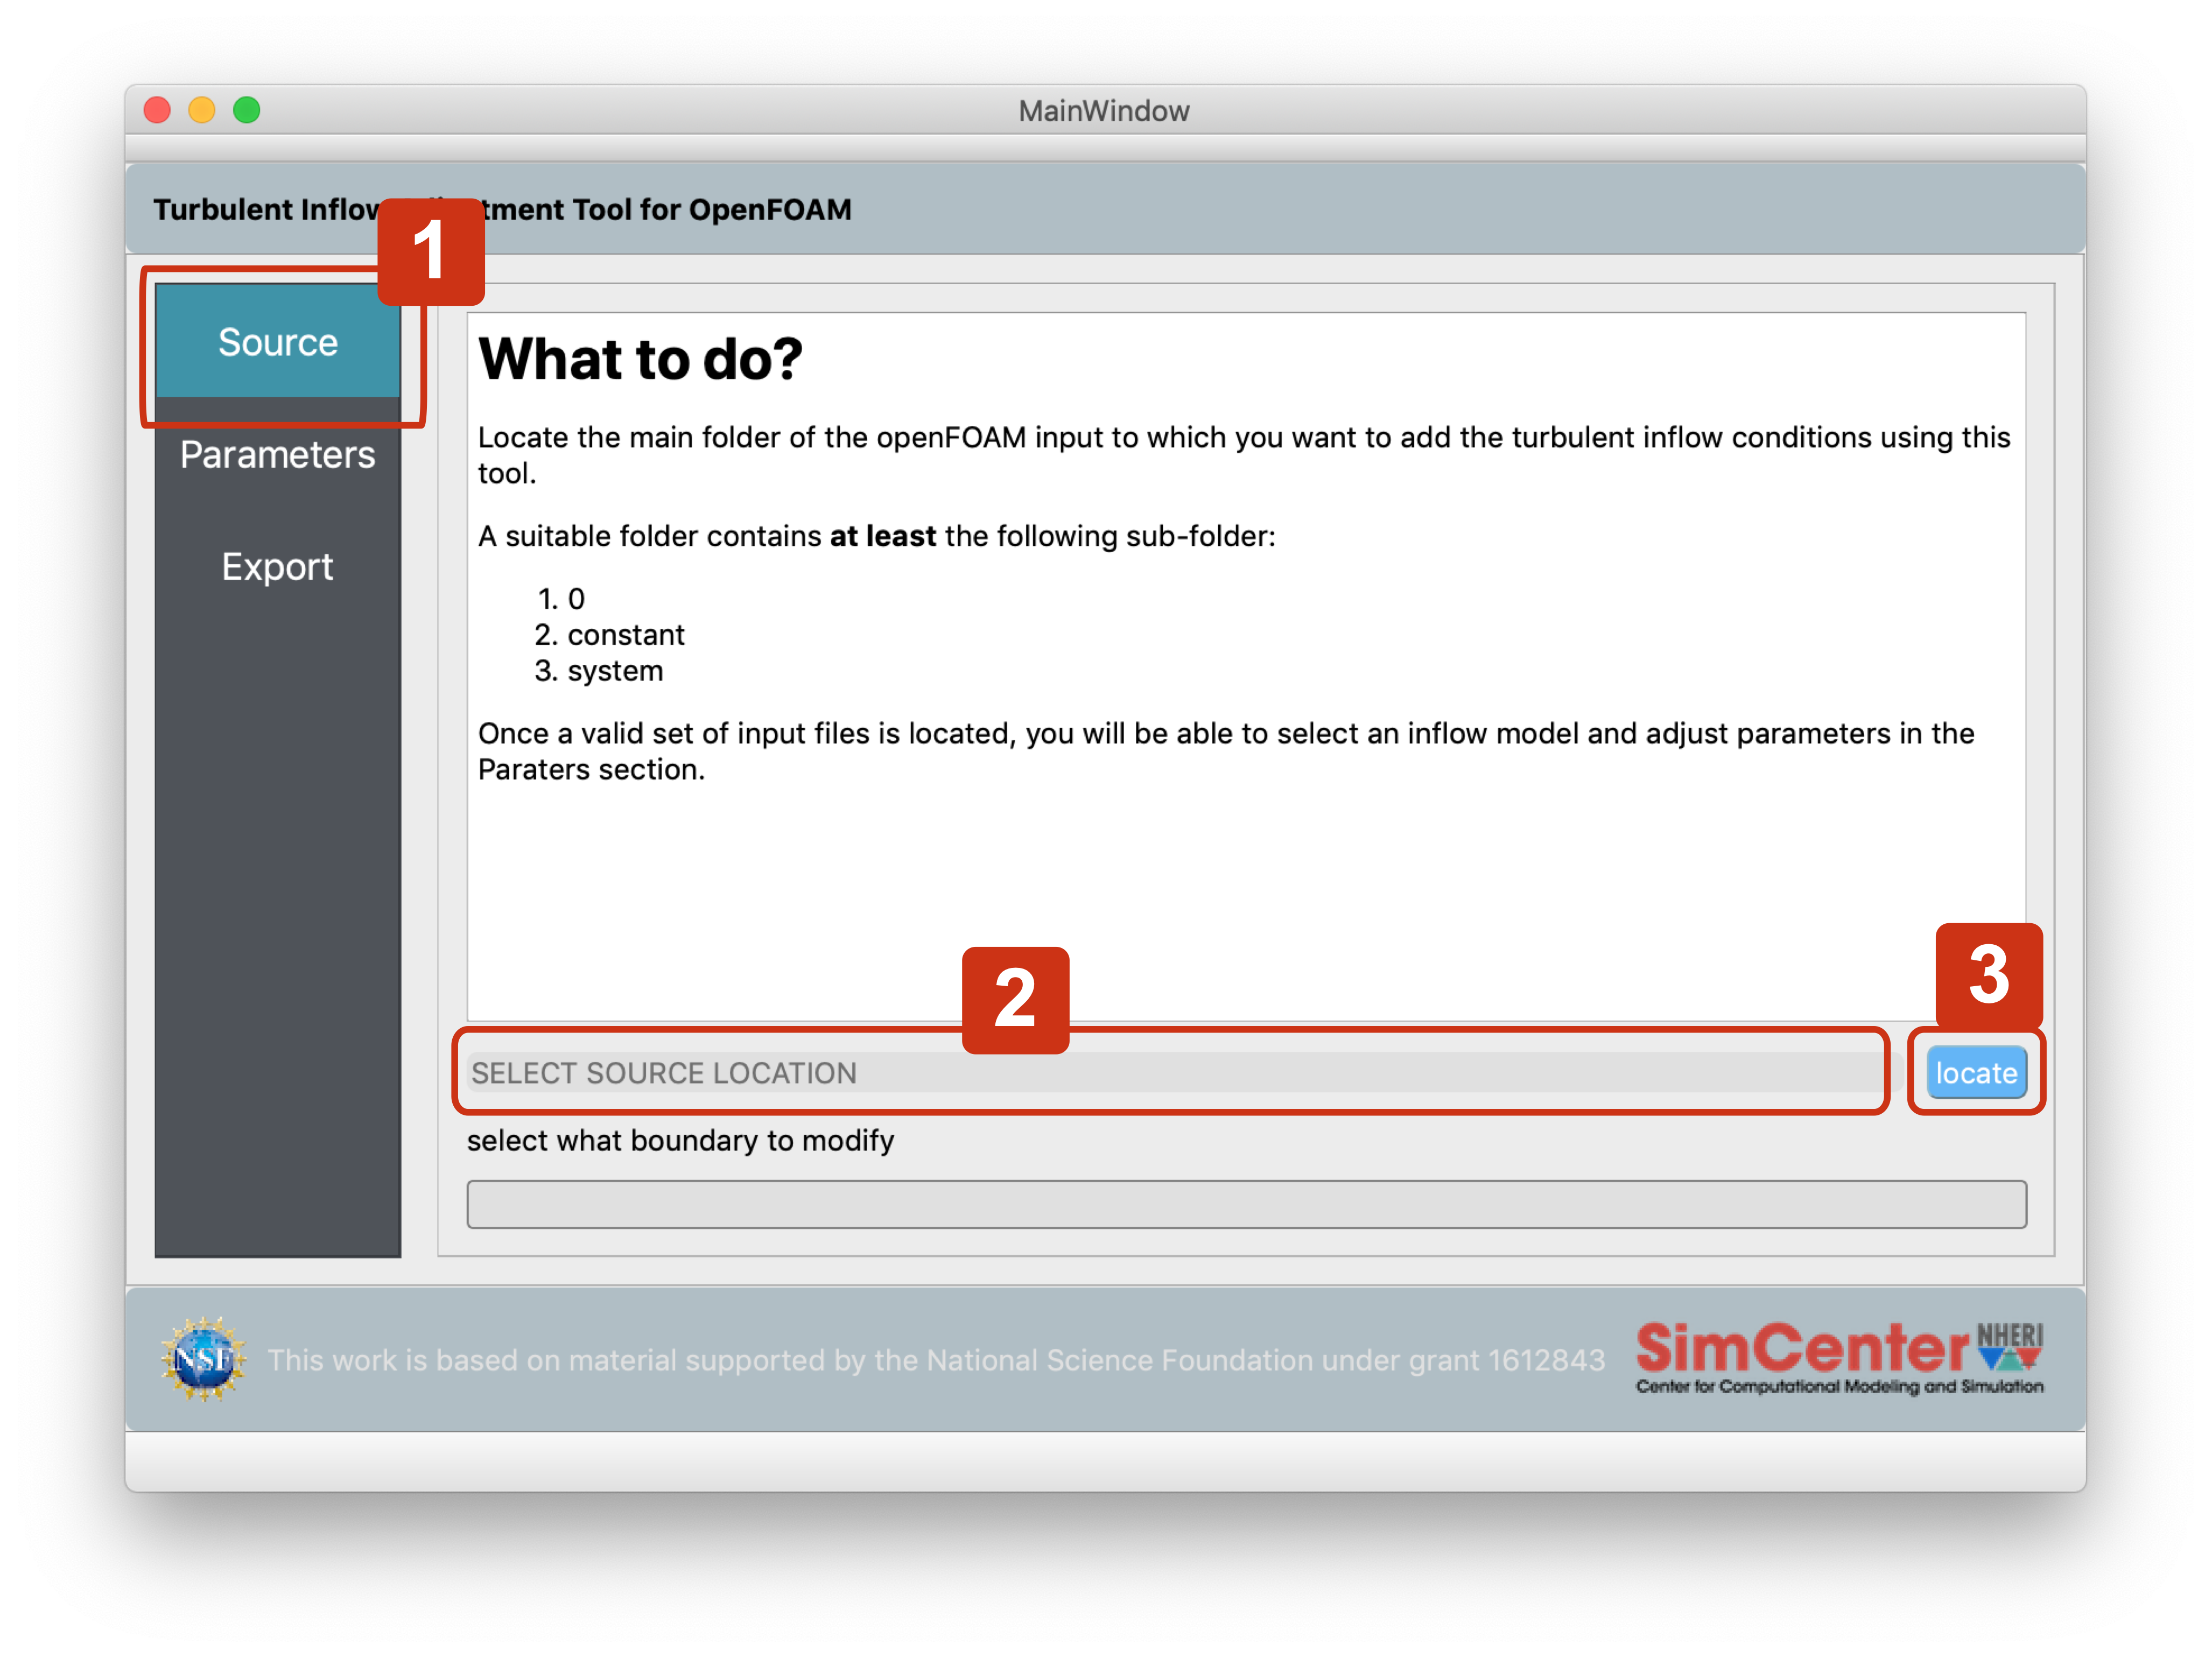
\includegraphics[width=0.90\hsize]{TInF-01.png}
		\vspace*{-1.5\baselineskip}
		\caption{Start page -- Source selection}
		\label{fig:TInF01}
	\end{center}
\end{figure}

\begin{figure}[ht]
	\begin{center}
		\vspace*{-1.0\baselineskip}
		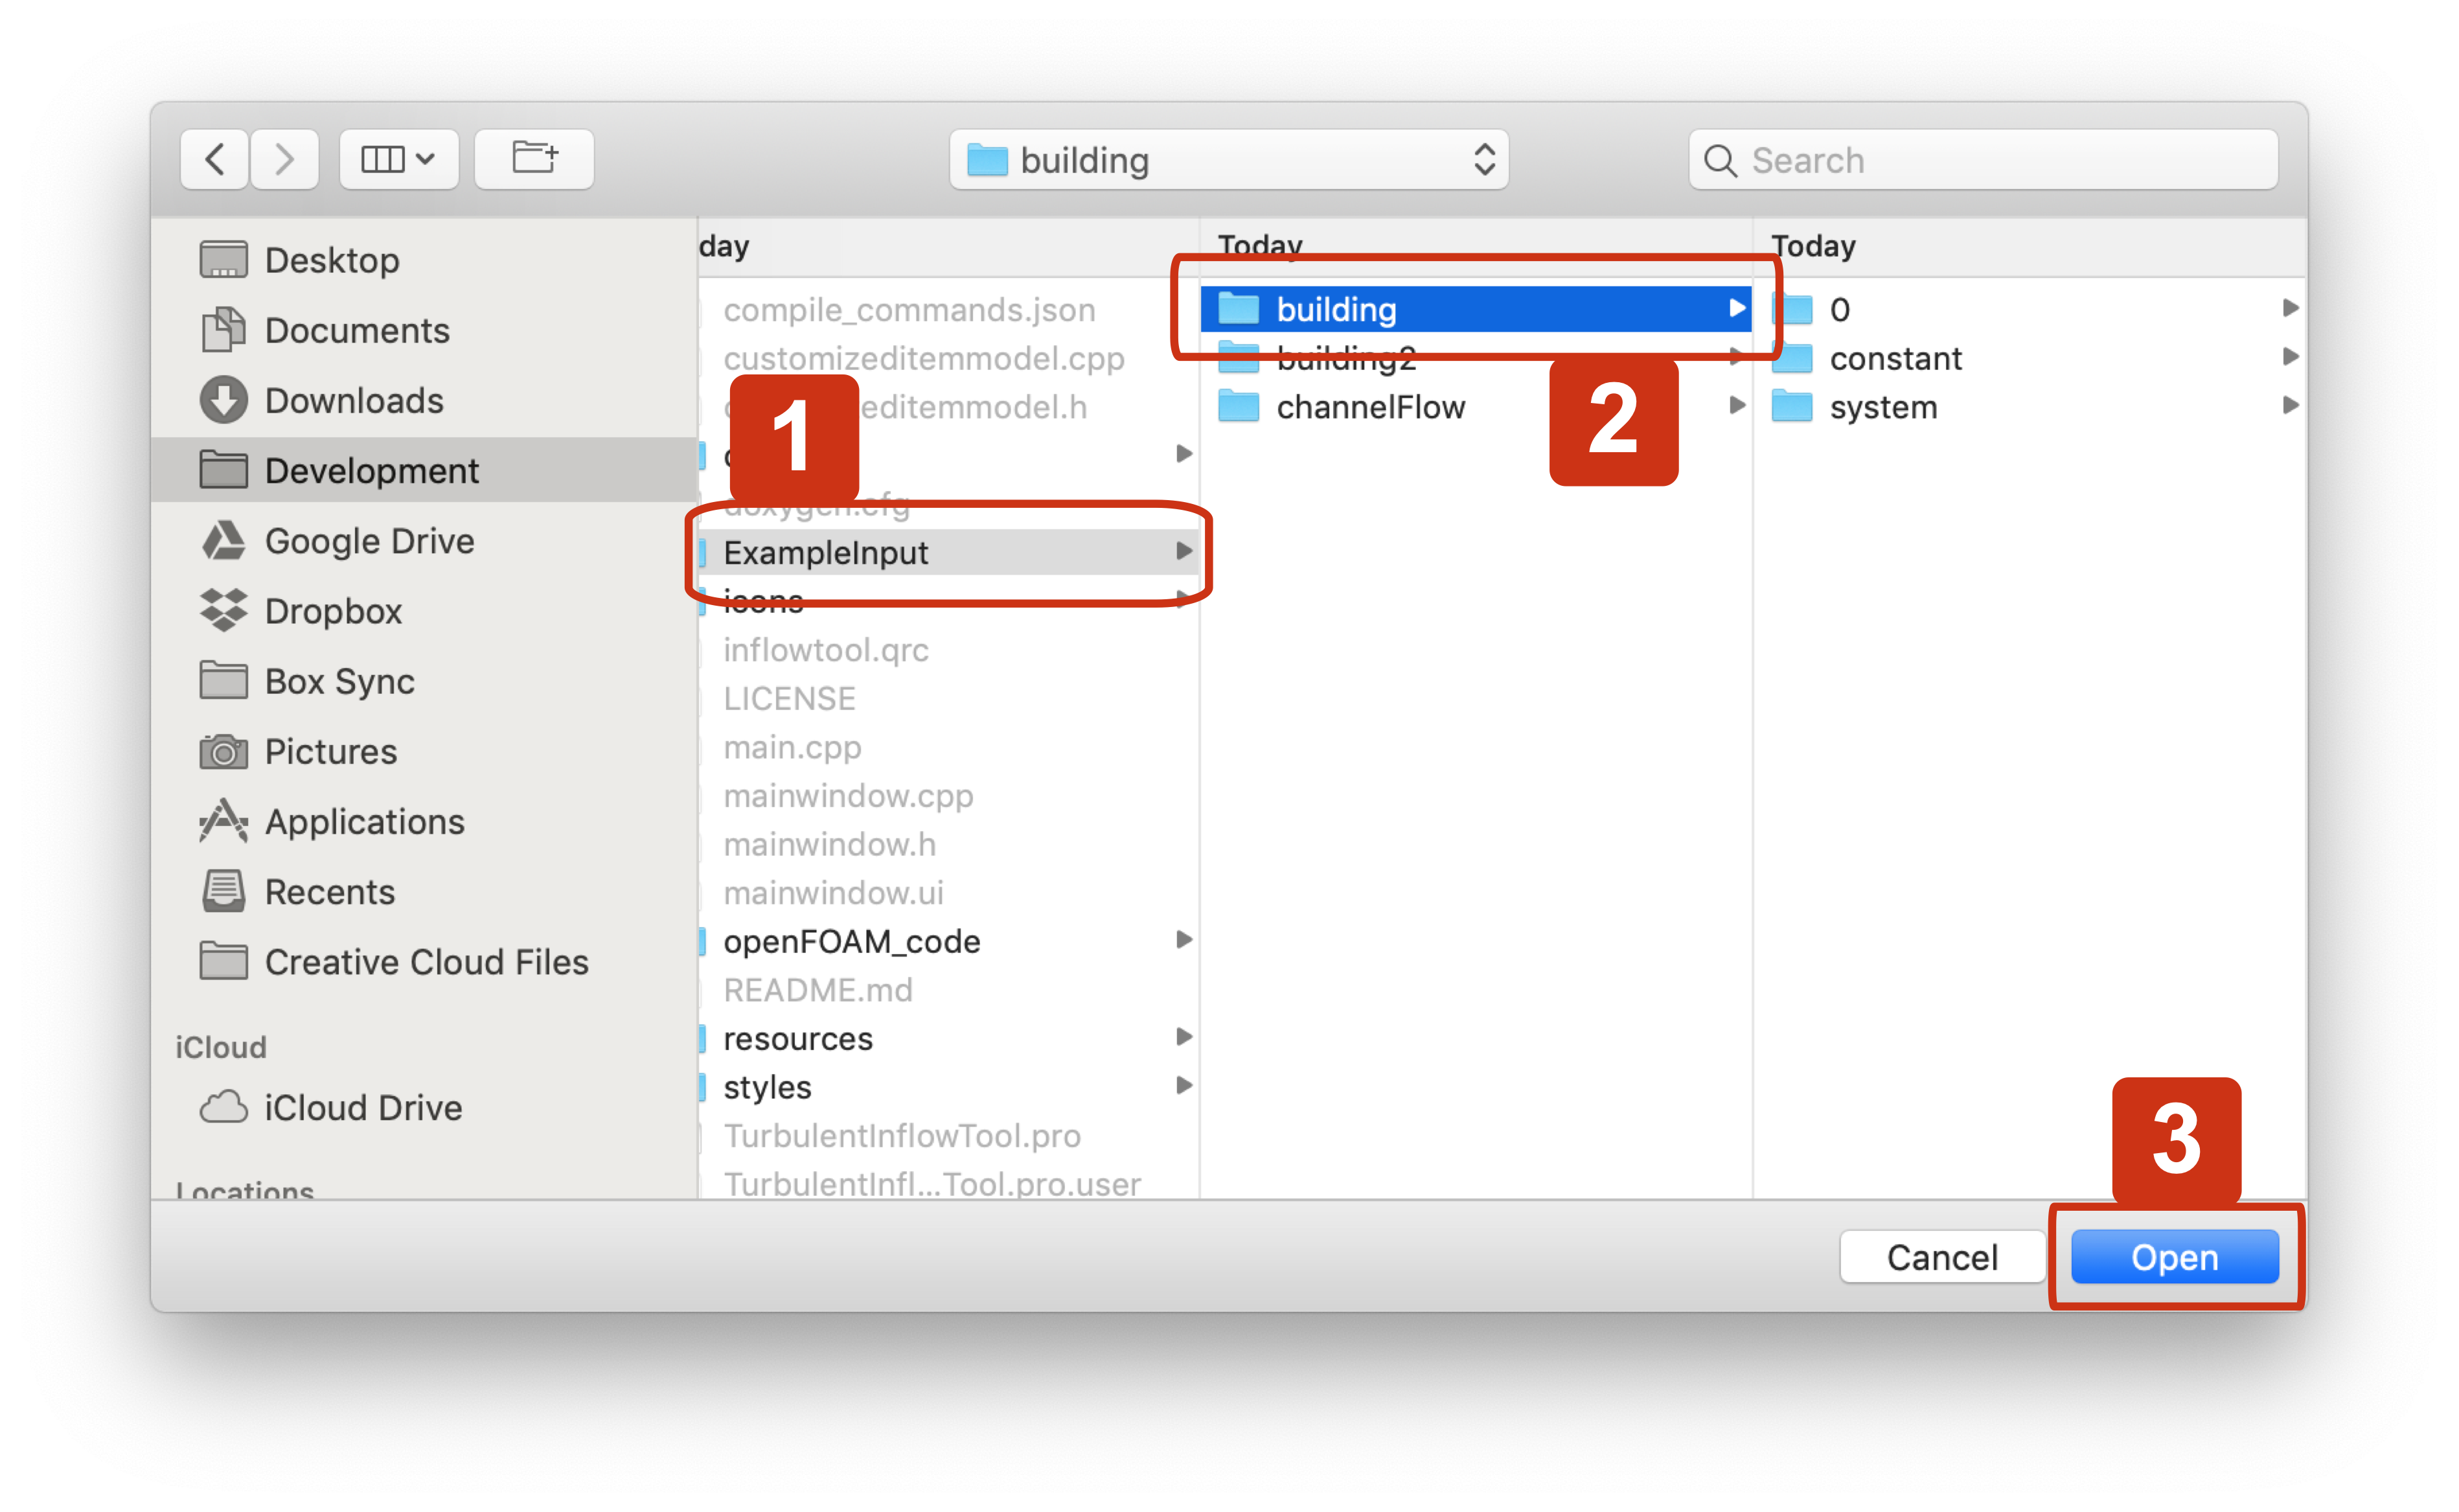
\includegraphics[width=0.90\hsize]{TInF-02.png}
		\vspace*{-1.5\baselineskip}
		\caption{Model tree selection (MacOS version shown, but similar on Windows systems)}
		\label{fig:TInF02}
	\end{center}
\end{figure}
Figure~\ref{fig:TInF02} shows a sample selection. The distribution comes with simple example input located in installed application folder.  Your provided input must at least contain the folders \texttt{0}, \texttt{constant}, and \texttt{system}. Navigate to the parent folder (Figure~\ref{fig:TInF02}, item~2) and press open (Figure~\ref{fig:TInF02}, item~3).

\begin{figure}[ht]
	\begin{center}
		%\vspace*{-1.0\baselineskip}
		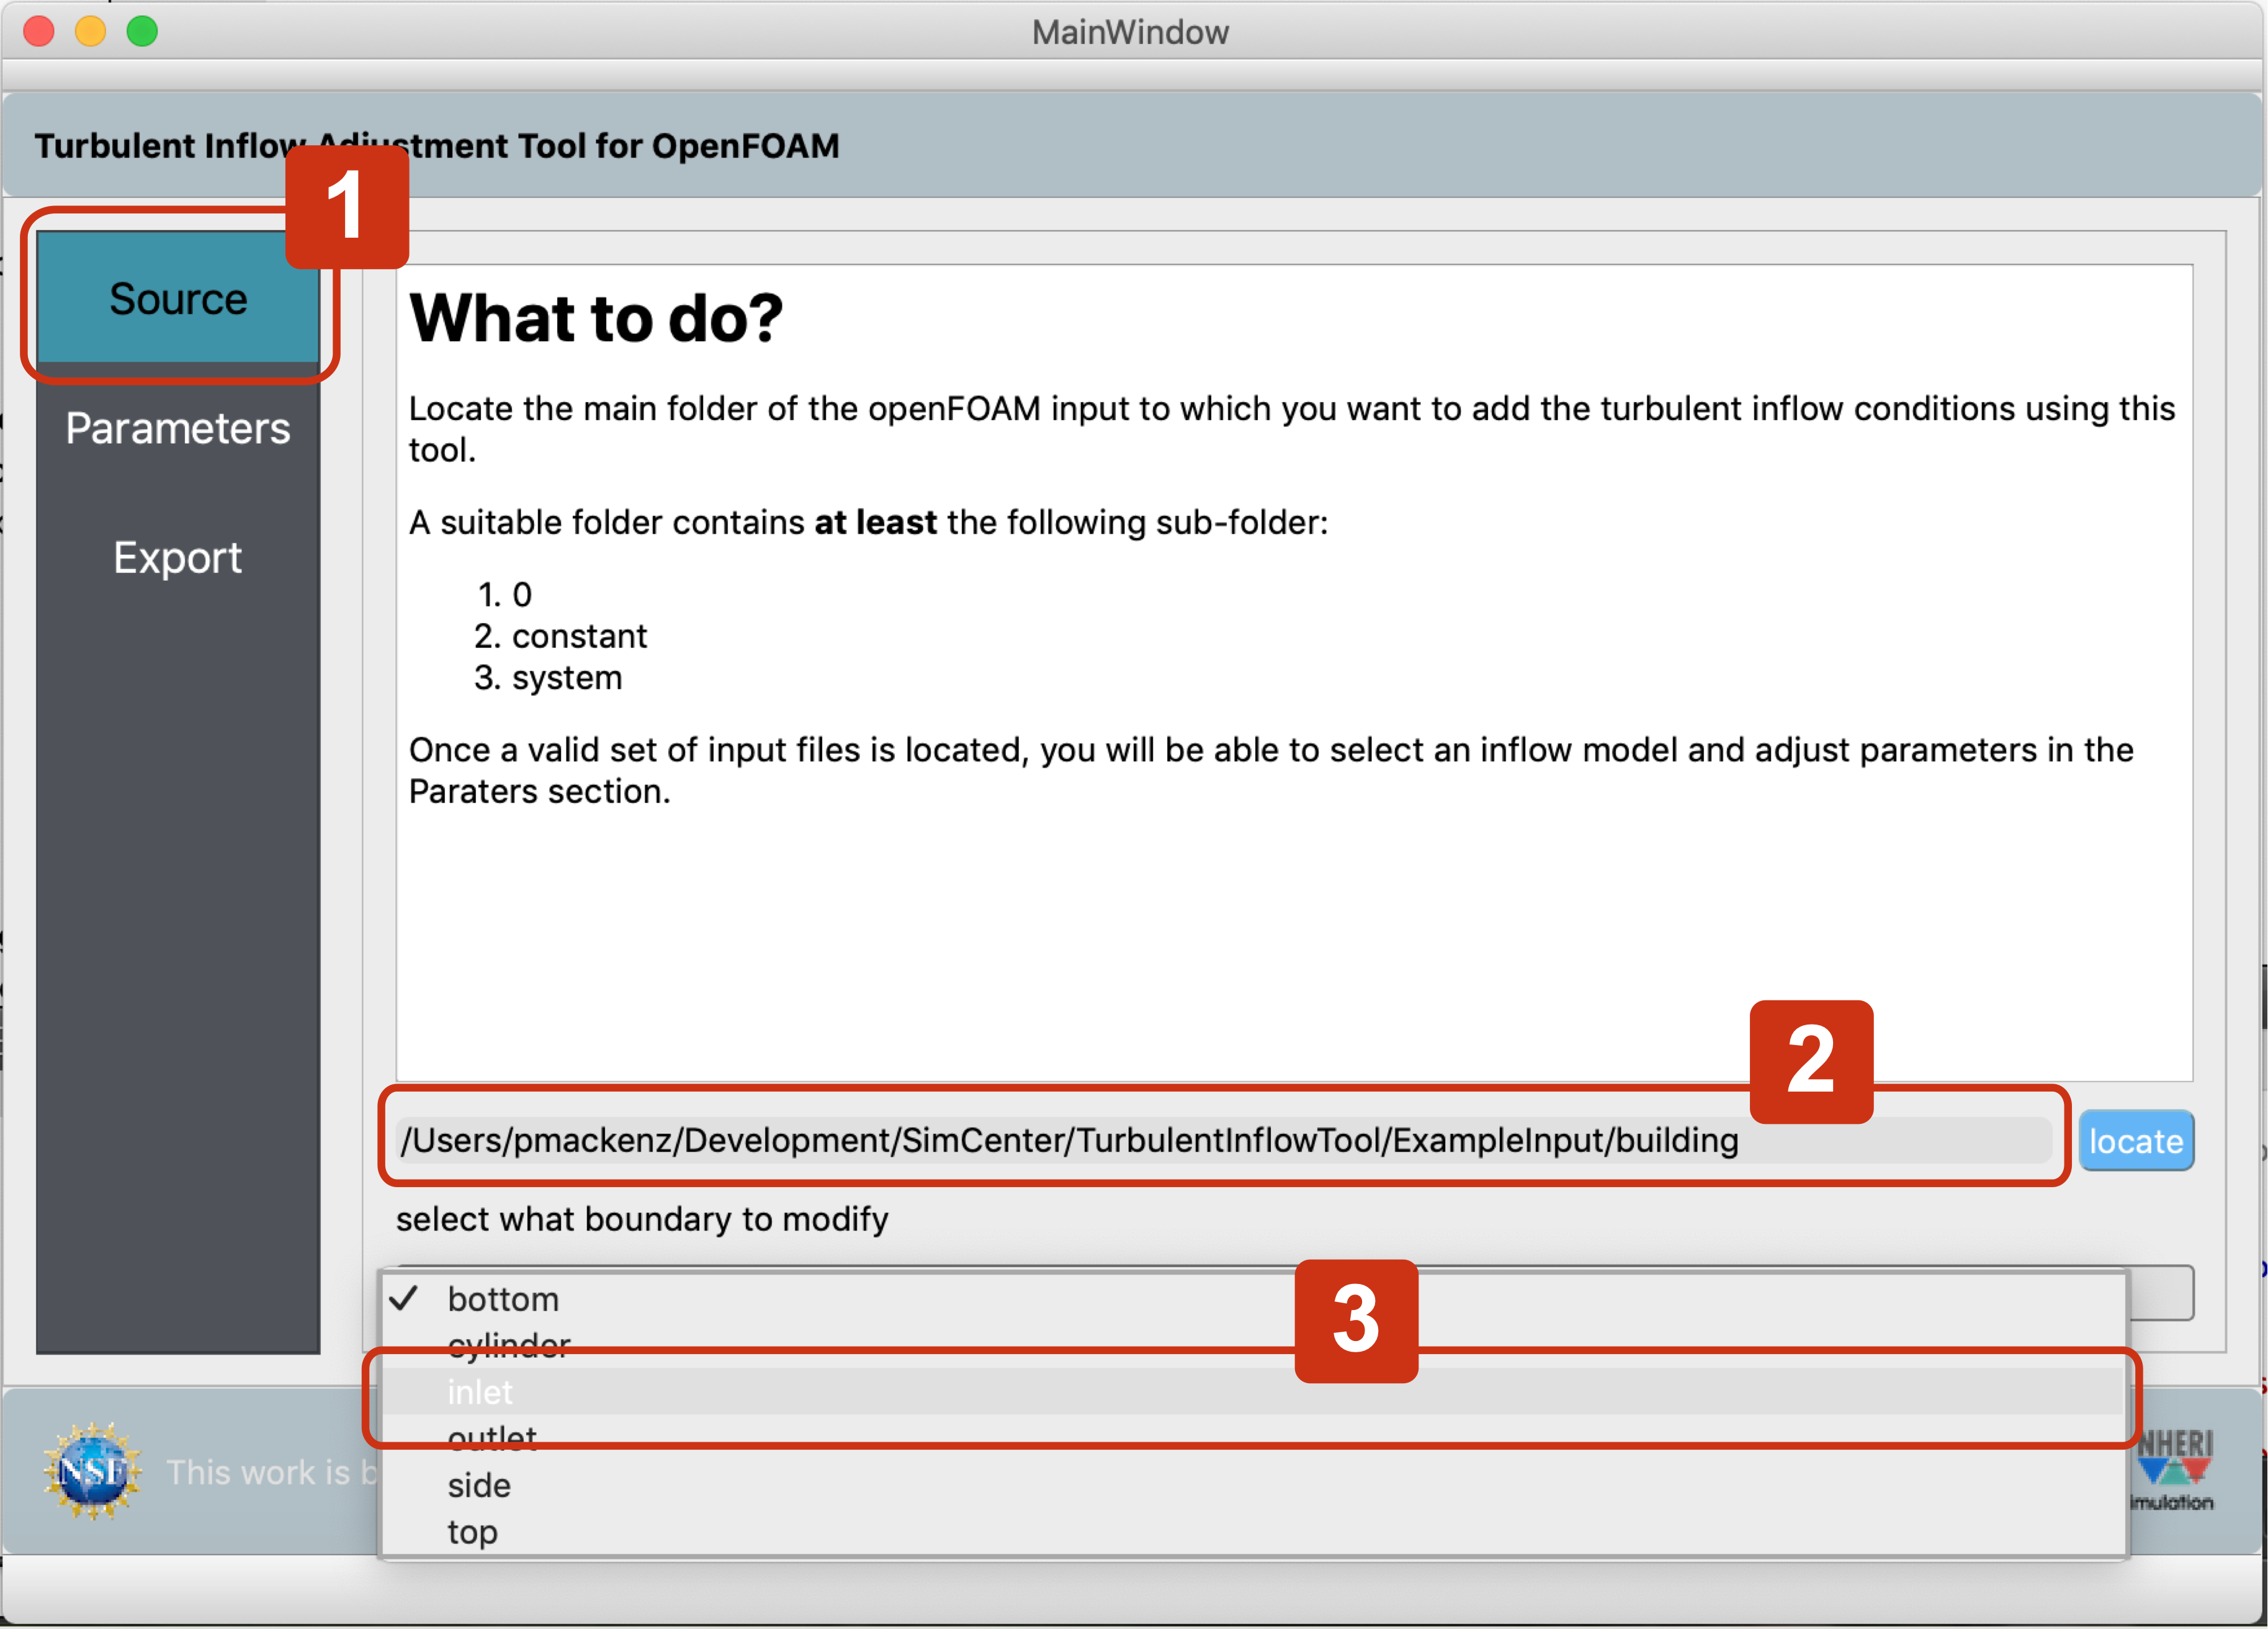
\includegraphics[width=0.90\hsize]{TInF-04.png}
		%\vspace*{-1.5\baselineskip}
		\caption{Boundary patch selection}
		\label{fig:TInF04}
	\end{center}
\end{figure}
The tool will display your selection (Figure~\ref{fig:TInF04}, item~2), parse your boundary condition definition and provide you with a list of found boundary patches (Figure~\ref{fig:TInF04}, item~3).  If your folder does not contain a parsable boundary patch definition, the folder will be displayed in red and no boundary patch selection will be offered.

Use the pull-down menu to select the proper boundary patch to which the turbulence inflow conditions will be applied.


\item[Step~2: Parameter Definition] 
In the Parameters tab (Figure~\ref{fig:TInF07} and  \ref{fig:TInF08}, item~1), first select the desired method.

\begin{figure}[htp]
	\begin{center}
		\vspace*{-1.0\baselineskip}
		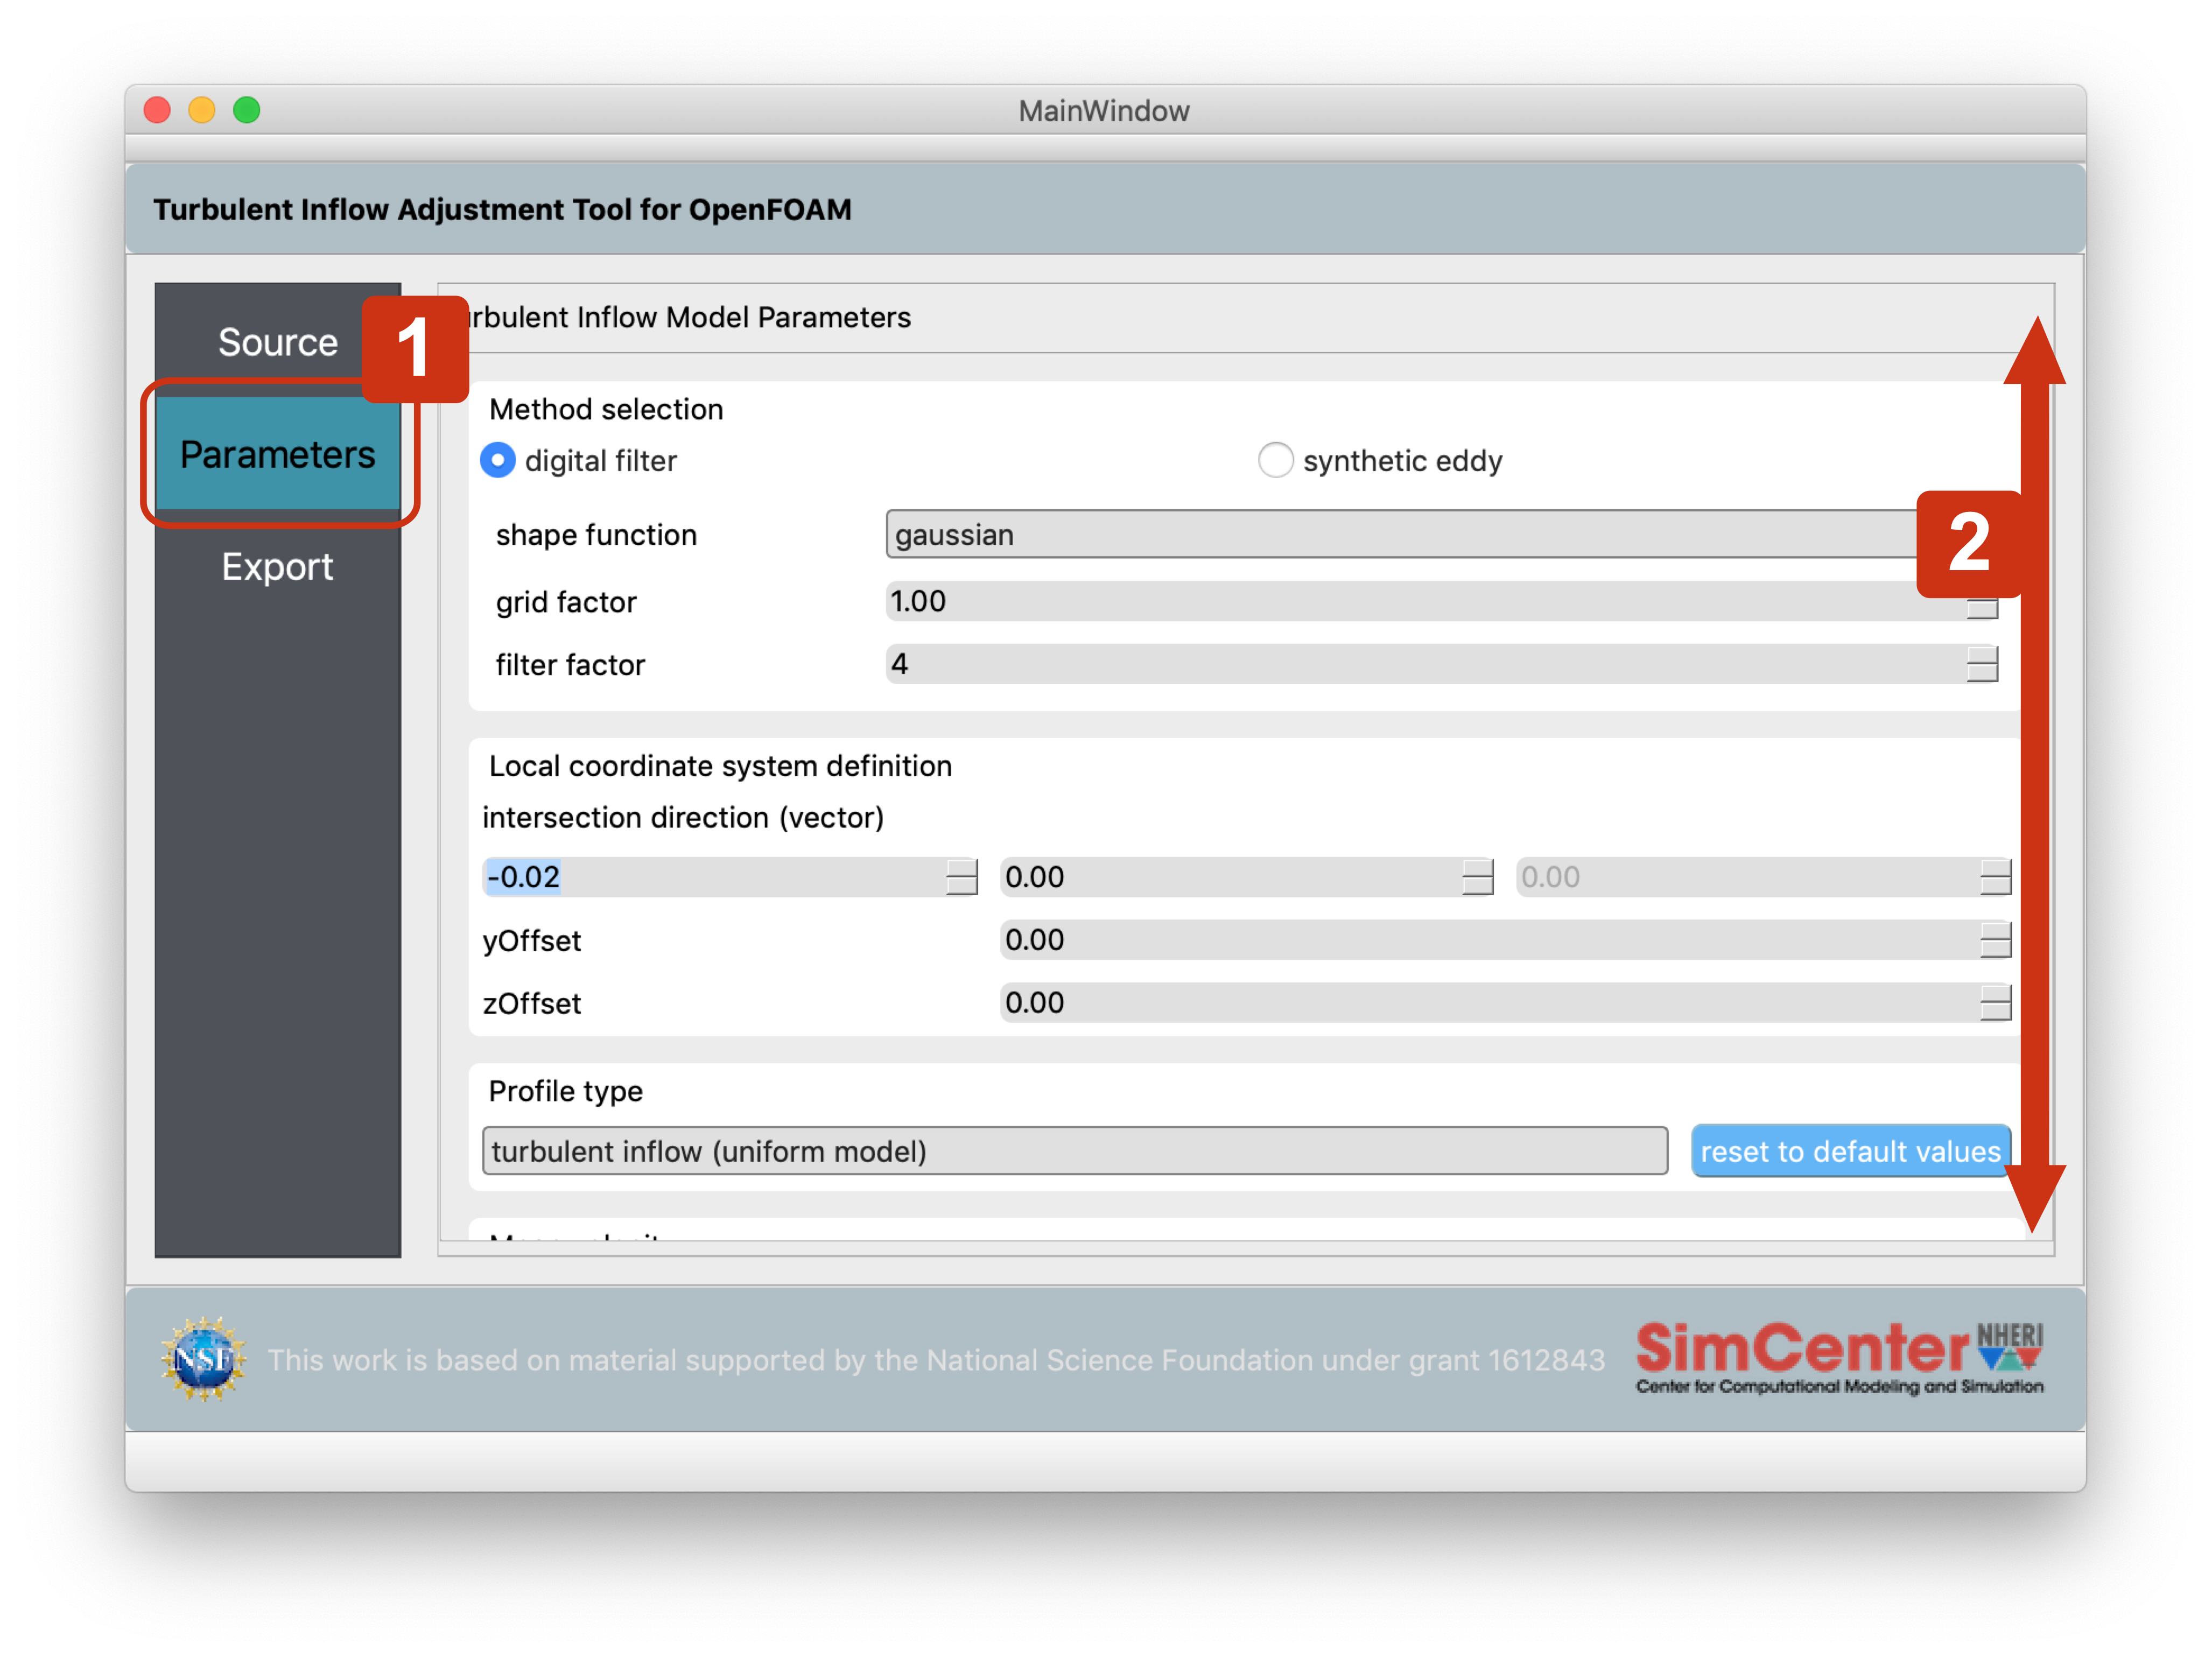
\includegraphics[width=0.90\hsize]{TInF-07.png}
		\vspace*{-1.5\baselineskip}
		\caption{Parameter selection tab -- top of page}
		\label{fig:TInF07}
	\end{center}
\end{figure}
\begin{figure}[htp]
	\begin{center}
		\vspace*{-1.0\baselineskip}
		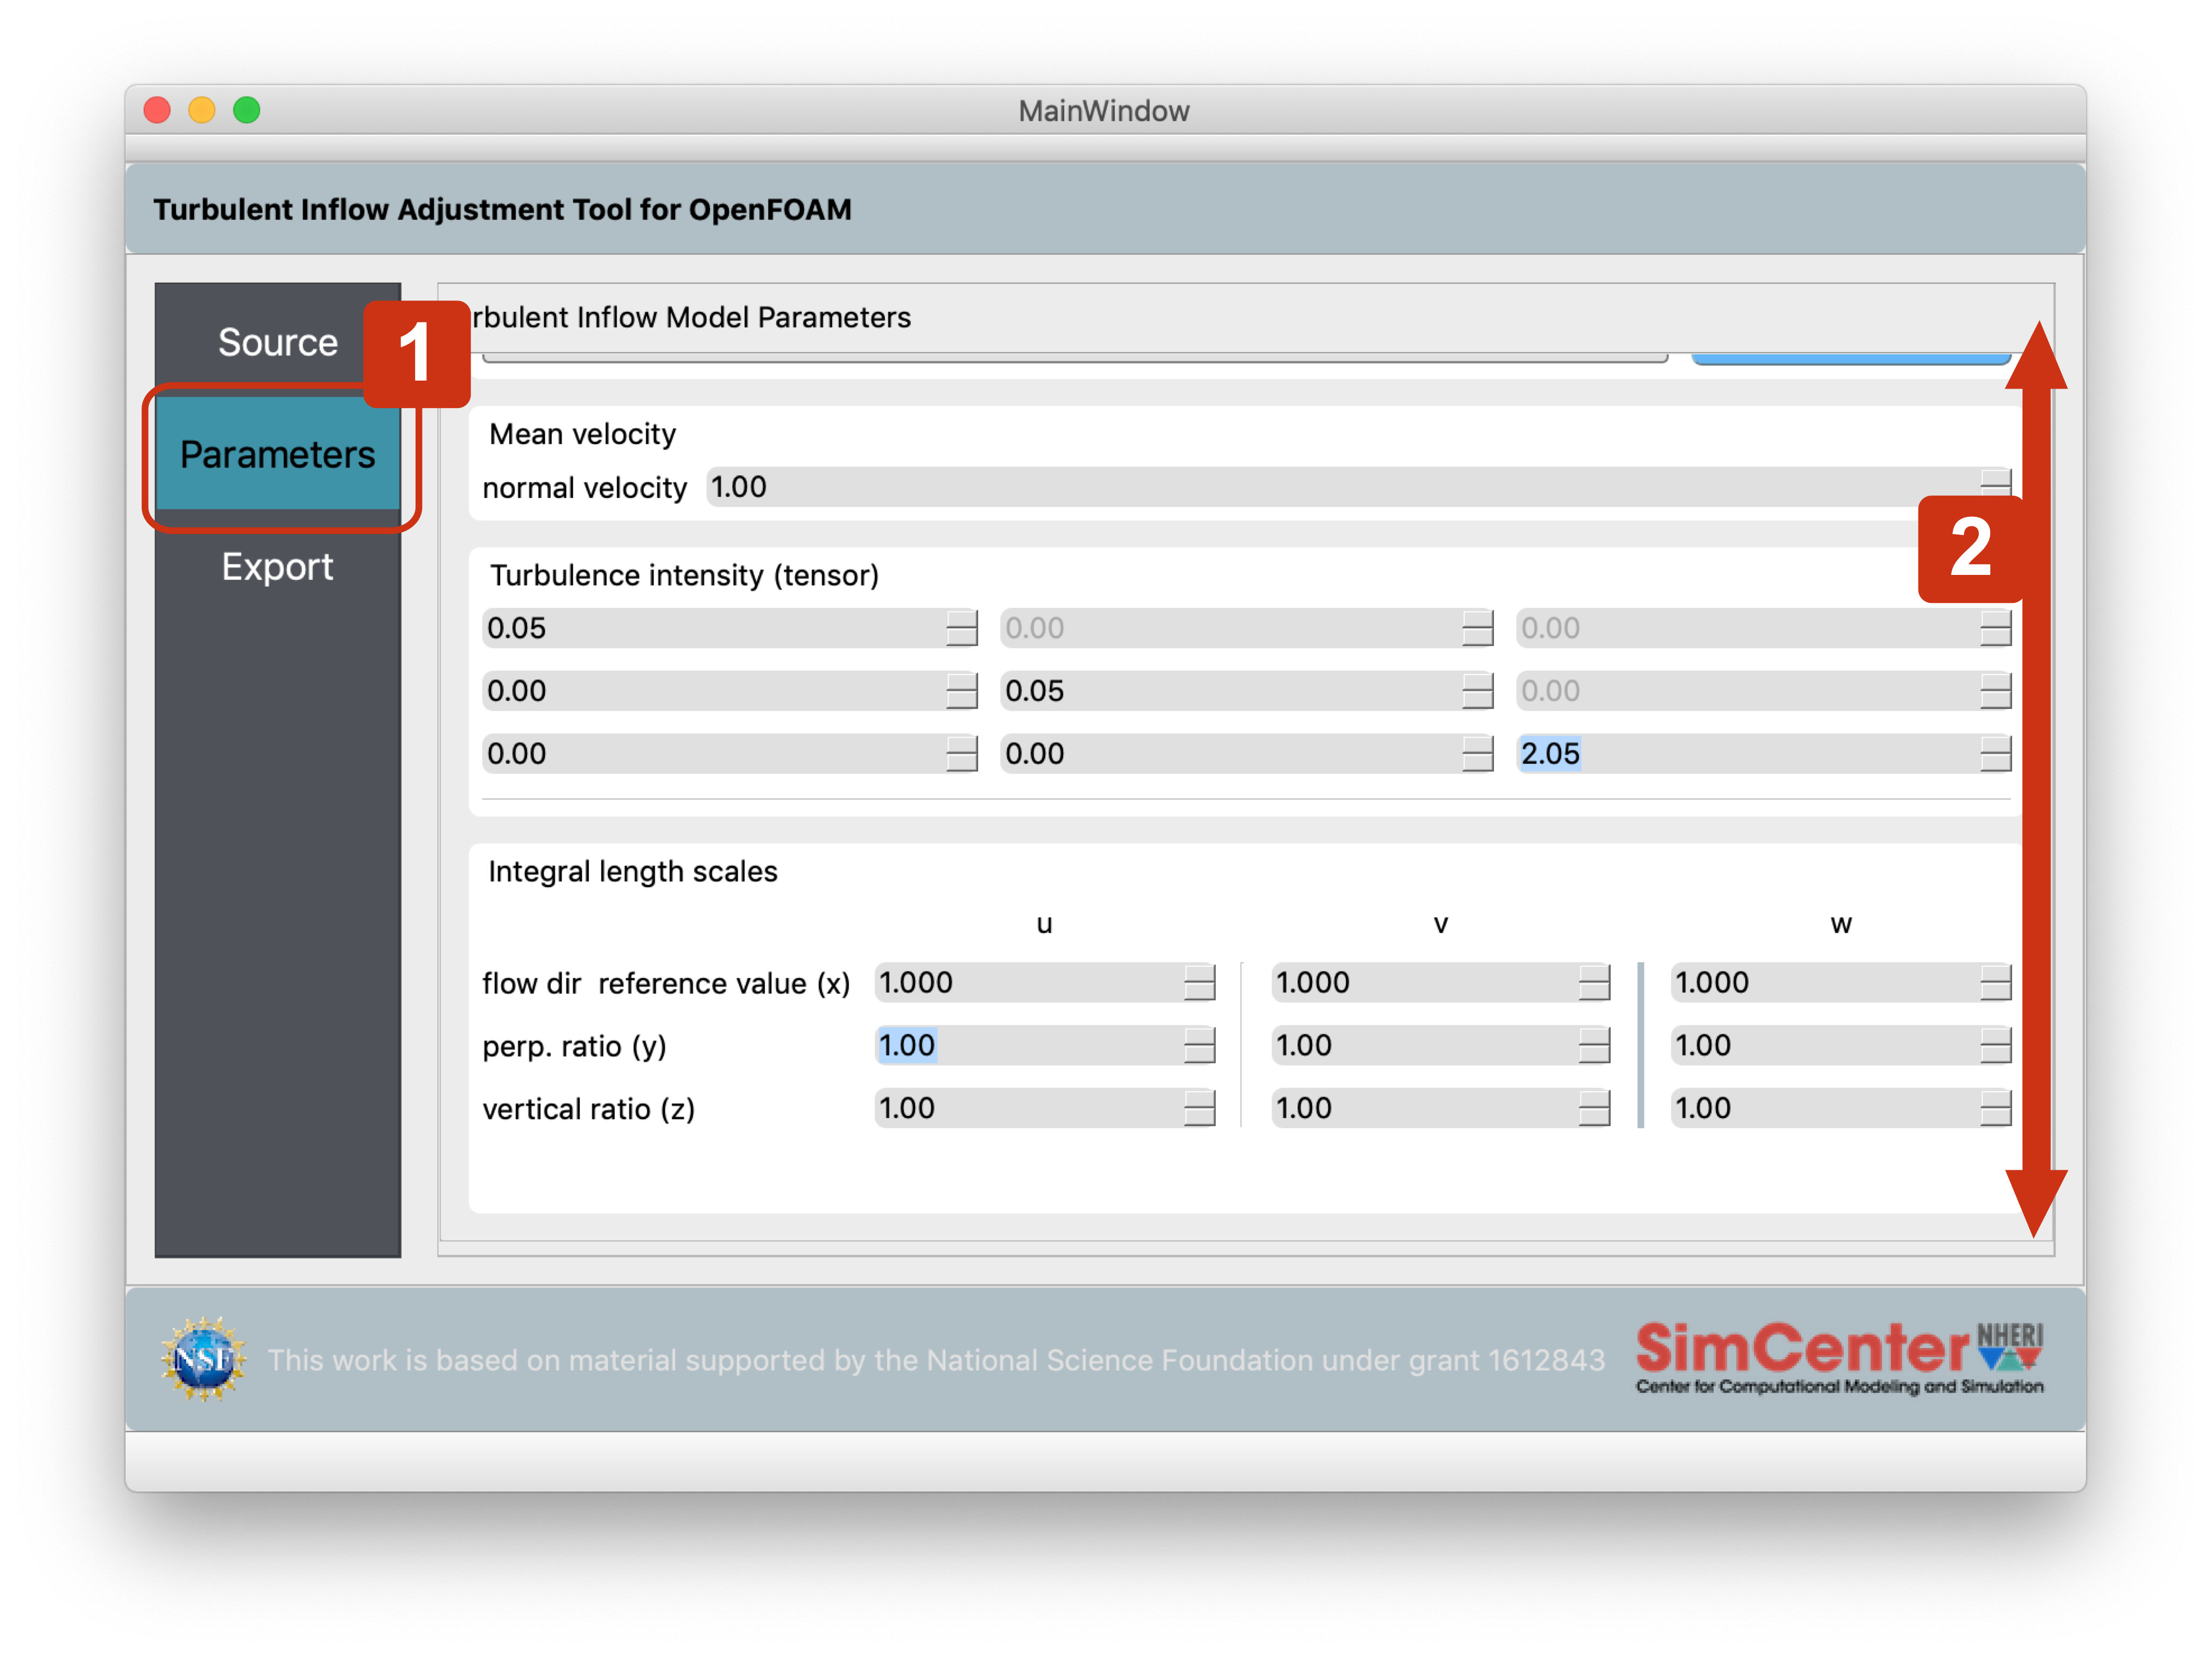
\includegraphics[width=0.90\hsize]{TInF-08.png}
		\vspace*{-1.5\baselineskip}
		\caption{Parameter selection tab -- bottom of page}
		\label{fig:TInF08}
	\end{center}
\end{figure}


Based on the selected method, additional parameters will be collected.  The particular parameters and their meaning are discussed in detail in Chapter~\ref{sec:TInF-theory}.
Depending on selected model and sub-options, as well as your screen size, you may need to scroll down to get access to all parameter fields (Figure~\ref{fig:TInF07} and  \ref{fig:TInF08}, item~2)  \footnote{WARNING: the window manager on MacOS is hiding any scroll bar until you attempt to slide the parameter fields up.}.

\item[Step~3: Export Changes to your Model] 

Once all parameters have been defined, you are ready to export the necessary changes to your model definition files.

\begin{figure}[h]
	\begin{center}
		\vspace*{-1.0\baselineskip}
		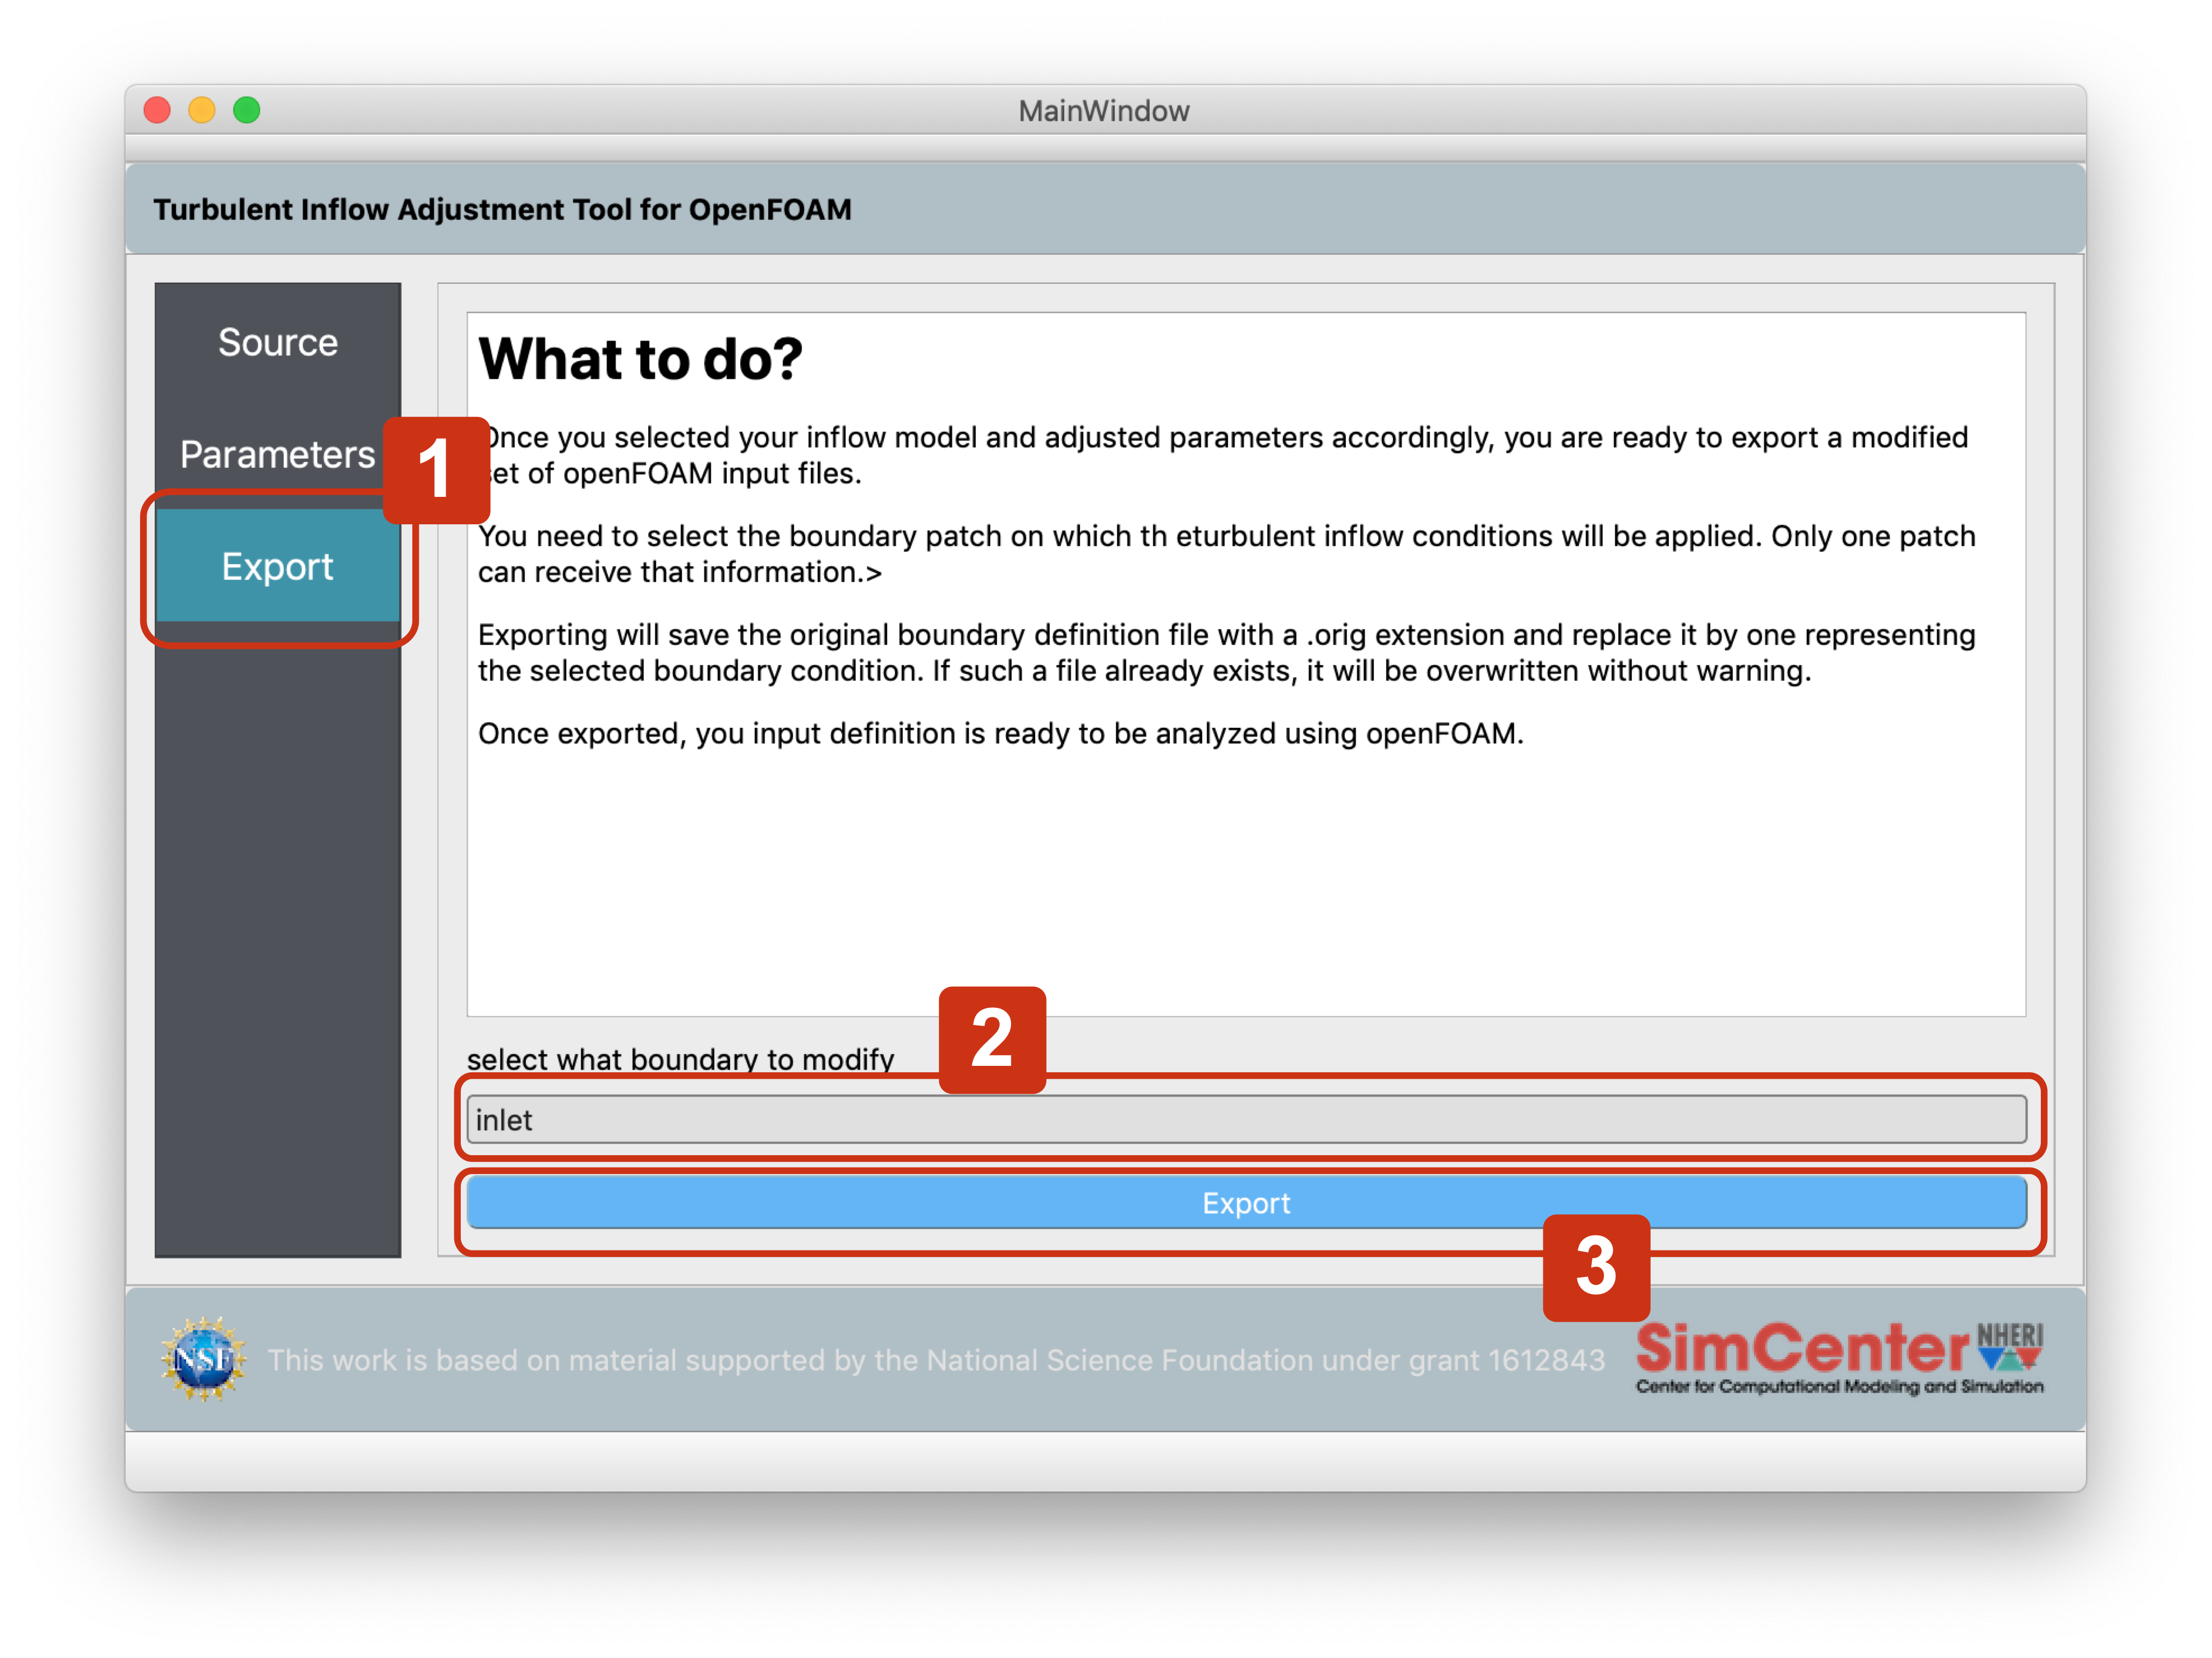
\includegraphics[width=0.90\hsize]{TInF-09.png}
		\vspace*{-1.5\baselineskip}
		\caption{Export panel}
		\label{fig:TInF09}
	\end{center}
\end{figure}

In the Export panel (Figure~\ref{fig:TInF09}, item~1), verify that the correct boundary patch is selected
(Figure~\ref{fig:TInF09}, item~2).
This is the same as what is selected in the Source panel (Figure~\ref{fig:TInF04}, item~3). Actually, those fields are linked and changes to either will automatically sync the other.

Once you are certain that the correct patch has been selected, press the Export button
(Figure~\ref{fig:TInF09}, item~3) to write the updated boundary definition files.  Existing files will be saved to name.orig.

\textbf{WARNING:} Only one copy of the original file will be made.  Subsequent exports will treat the previously modified files as the source to be saved.  Any older versions will be overwritten without further warning.


\end{description}




\chapter{Theory and Implementation}
\subsection{Introduction}
\label{sec:TInF-theory}

In computational wind engineering (CWE), generation of inflow turbulence satisfying prescribed mean-velocity profiles, turbulence spectra, spatial and temporal correlations is of great importance for the accurate evaluation of wind effects on buildings and structures. More specifically, the task is to generate a turbulent velocity field $\boldsymbol{u}(\boldsymbol{x},t)$ with the form

\begin{equation}
\boldsymbol{u}(\boldsymbol{x},t) = \boldsymbol{U}(\boldsymbol{x},t)+\boldsymbol{u}'(\boldsymbol{x},t)
\end{equation}

\noindent where $\boldsymbol{U}(\boldsymbol{x},t)$ and $\boldsymbol{u}'(\boldsymbol{x},t)$ are the mean and fluctuating velocities at the position $\boldsymbol{x}$. The turbulent velocity field $\boldsymbol{u}$ and its fluctuation $\boldsymbol{u}'$ need to satisfy a number of properties which are list below:

\begin{itemize}
\item $\boldsymbol{u}'$ should be spatially and temporally correlated.
\item $\boldsymbol{u}'$ needs to have prescribed Reynolds stresses tensor $R_{ij}(\boldsymbol{x}) = \overline{u_i'u_j'}(\boldsymbol{x})$ where $u_i'$ ($i=1,2,3$) is the $i$-th component of $\boldsymbol{u}'$  and the over line denotes the time average.
\item $\boldsymbol{u}'$ needs to have prescribed integral length scales $L_{ij}(\boldsymbol{x},\boldsymbol{e})$
\begin{equation}
L_{ij}(\boldsymbol{x},\boldsymbol{e}) = \int_{0}^{\infty} \rho_{ij}(\boldsymbol{x},r\boldsymbol{e})\ \mathrm{d}r,
\end{equation}
\noindent where $\rho_{ij}(\boldsymbol{x},\boldsymbol{e})$ is the correlation function given by
\begin{equation}
\rho_{ij}(\boldsymbol{x},\boldsymbol{e}) = \frac{\overline{u_i'(\boldsymbol{x},t)u_j'(\boldsymbol{x}+\boldsymbol{e},t)}}{\overline{u_i'(\boldsymbol{x},t)u_j'(\boldsymbol{x},t)}}.
\end{equation}
\item $\boldsymbol{u}$ should fulfil the divergence free constraint $\nabla \cdot \boldsymbol{u} = 0$.
\item $\boldsymbol{u}'$ should have prescribed correlation functions $\rho_{ij}(\boldsymbol{x},\boldsymbol{e})$ or spectra.
\end{itemize}

\noindent Several methodologies have been proposed for this purpose which can be classified into three general categories: precursor simulation methods, recycling methods and synthetic methods. Compared with precursor simulation and recycling methods, the synthetic methods in general offer a more practical and relatively efficient approach to generate inflow turbulence, and is therefore chosen as the subject of this section. Research activities on synthetic turbulence generation have been vigorous over the past decades and have branched out into several categories of techniques \cite{wu2017}, including the synthetic random Fourier method \cite{kraichnan1970, hoshiya1972}, the synthetic digital filtering method \cite{klein2003} and the synthetic eddy methods \cite{jarrin2006}. A brief introduction regarding to these techniques is given below and emphasis is placed on their abilities to capture the statistical characteristics as well as the spatial and temporal coherence of turbulence. Also note that since real turbulence is very complex, in most cases, not all of the above listed features can be fulfilled. There is always some adaptation time required for the artificial turbulence to evolve into real turbulence. Fulfilling the properties above with the synthetic turbulence is important to minimize the adaptation time or length.

\subsection{Synthetic Random Fourier Method}

The so-called synthetic random Fourier method (SRFM) attempts to model turbulent flow field indirectly by imposing constraints on uncorrelated random fields through an energy spectrum to account for the spatial and temporal correlations, which can be further classified into two groups. 
The first group of the SRFM was based on the pioneering work in \cite{hoshiya1972} and \cite{shinozuka1972} on the simulation of multi-correlated random processes using a weighted amplitude wave superposition (WAWS) method. This approach has an advantage that both the targeted power- and cross-spectra can be imposed in the generation process so that the prescribed target characteristics can be maintained. A major drawback of this method is that the generated turbulence does not satisfy the continuity equation of the flow, or in other words, the divergence-free condition is not guaranteed. As a consequence it would take enormous effort for the solver to enforce the continuity by correcting the turbulence inflow inserted into the computational domain, and the statistical characteristics of the corrected flow field differs from the target values.

The second group of the SRFM was initiated by the work in \cite{kraichnan1970} on divergence-free homogeneous isotropic turbulence synthesis through the superposition of random harmonic functions. \cite{smirnov2001} took a step forward by combing Kraichnan's technique with scaling and orthogonal transformation operations in a procedure known as the random flow generation (RFG) which allows to generate inhomogeneous and anisotropic turbulence. However the scaling operation introduced in the RFG technique can result in a velocity field that is not divergence-free for inhomogeneous turbulence. Modifications to enforce the divergence-free constraint for inhomogeneous turbulence was discussed in \cite{yu2014}. A major drawback of RFG technique is that the power-spectra of the generated turbulence only follows Gaussian's spectra model, so it is not suitable for simulating flows in atmospheric boundary layer. \cite{huang2010} revisited Kraichnan's method and proposed a technique called DSRFG (for discretizing and synthesizing random flow generation) which allows to generate turbulent inflow from any prescribed spectrum. Instead of using the scaling and orthogonal transformation, the anisotropy of turbulence is realized by modifying the distribution strategy of the wave vector in Kraichnan's original method. A drawback of the DSRFG technique is that it produces fluctuating velocities with high correlation due to the fact that in this method the spatial correlation is modelled by a parameter which is not a function of frequency but a constant value. Inspired by the DSRFG method, \cite{castro2017} proposed some modifications to this technique to obtain the velocity field that had a better match with the target turbulent statistics. This method, known as modified discretizing and synthesizing random flow generation (MDSRFG), is capable of removing the dependence of statistic quantities of synthetic turbulence on spectra discretization resolution. \cite{aboshosha2015} also proposed a technique called consistent discrete RFG (CDRFG) to accurately model the target spectra and the coherence function. In both two methods mentioned above, the parameter that characterizes the spatial correlation is expressed as a function of frequency to account for the damping of coherence with the increase of frequency. An attractive feature of second group of SRFM is that the generation procedures are usually independent at each point and each time-instant so that it can be easily accelerated by conducting parallel computation, although the generated random flow may not satisfy the continuity equation. 


\subsection{Synthetic Eddy Method}\label{section3}

The synthetic eddy method (SEM) initiated by \cite{jarrin2006} is based on the classical view of turbulence as a superposition of the representative coherent eddies. In the SEM, the flow is assumed to consist of randomly distributed turbulent spots, and each turbulent spot is modelled by a three-dimensional shape function with compact support and satisfies a proper normalization condition. The spots are then assumed to be convected through an inlet plane with a reference velocity using Taylor's frozen turbulence hypothesis. The resulting inflow turbulence is then reconstructed using the method proposed by to recover the desired statistical characteristics and to account for the conditions of inhomogeneity and anisotropy. The choice of the shape function plays an important role in the SEM since it is directly related to the two-point autocorrelation function, and consequently the power spectrum of the synthetic turbulence. Enforcement of the continuity condition in the SEM was discussed in \cite{poletto2013}.

A brief introduction on the SEM presented by \cite{jarrin2006} is given as follows. To start with, the turbulent spot mentioned above can be represented as eddies defined by shape function $f$ which has a compact support on $[-1,1]$ and has the normalization

\begin{equation} \label{normalization}
\int_{-1}^1 f^2(x) \mathrm{d}x = 1
\end{equation}

\noindent The inflow plane on which we want to generate the synthetic turbulence with the SEM is basically a finite set of points $S = \{\boldsymbol{x}_1,\boldsymbol{x}_2,\ldots,\boldsymbol{x}_s\}$. The first step is to create a box of eddies $B$ surrounding $S$ which is going to contain the synthetic eddies. It is defined by

\begin{equation}
B = \big\{(x_1,x_2,x_3)\in \mathbb{R}^3: x_{i,\text{min}}<x_i<x_{i,\text{max}}\big\}
\end{equation}

\noindent where

\begin{equation}
x_{i,\text{min}} = \text{min}(x_i-\sigma_i(\boldsymbol{x})), \quad x_{i,\text{max}} = \text{max}(x_i+\sigma_i(\boldsymbol{x})), \quad \boldsymbol{x}\in S
\end{equation}

\noindent The volume of the box of eddies is noted by $V_B$. In the synthetic eddy method, the velocity signal generated by $N$ eddies has the representation

\begin{equation} \label{SEMvelocity}
u_i(\boldsymbol{x}) = U_i(\boldsymbol{x}) + \frac{1}{\sqrt{N}}\sum_{k=1}^N a_{ij} \epsilon_j^k f_{\boldsymbol{\sigma}(\boldsymbol{x})}(\boldsymbol{x}-\boldsymbol{x}^k)
\end{equation}

\noindent where $\boldsymbol{x}$ represent the coordinates of computational points and $\boldsymbol{x}^k$ represent the coordinates of eddies. The coefficient $a_{ij}$ results from the Cholesky decomposition of a prescribed Reynolds stress tensor $R_{ij}$

\begin{equation} \label{LundCoefficients}
\left(\begin{matrix}
\sqrt{R_{11}} & 0 & 0 \\
R_{21}/a_{11} & \sqrt{R_{22}-a_{21}^2} & 0 \\
R_{31}/a_{11}  & (R_{32}-a_{21}a_{31})/a_{22} & \sqrt{R_{33}-a_{31}^2--a_{32}^2}
\end{matrix}\right)
\end{equation}

\noindent The coefficient $\epsilon_j^k$ ($j=1,2,3$) is is the uniformly random intensity factor of values $+1$ or $-1$, and $f_{\boldsymbol{\sigma}(\boldsymbol{x})} (\boldsymbol{x}-\boldsymbol{x}^k)$ is the velocity distribution at $\boldsymbol{x}$ of the eddy located at $\boldsymbol{x}^k$ defined as follows:

\begin{equation} \label{velocityShape}
f_{\boldsymbol{\sigma}(\boldsymbol{x})} (\boldsymbol{x}-\boldsymbol{x}^k) = \sqrt{\frac{V_B}{\sigma_1\sigma_2\sigma_3}}f\left(\frac{x_1-x_1^k}{\sigma_1}\right)f\left(\frac{x_2-x_2^k}{\sigma_2}\right)f\left(\frac{x_3-x_3^k}{\sigma_3}\right)
\end{equation}

\noindent where $\boldsymbol{\sigma}=(\sigma_1,\sigma_2,\sigma_3)^T$. The position of the eddies $\boldsymbol{x}^k$ before the first time step are independent from each other and taken from a uniform distribution over the box of eddies $B$. The eddies are convected through the box of eddies $B$ with the mean velocity $\boldsymbol{U}(\boldsymbol{x})$. At each time step, the new position of eddy $k$ is given by

\begin{equation}
\boldsymbol{x}^k(t+\varDelta t) = \boldsymbol{x}^k(t)+\boldsymbol{U}(\boldsymbol{x}^k)\varDelta t
\end{equation}

\noindent where $\varDelta t$ is the time step of the simulation. If an eddy $k$ is convected out of the box $B$, then it is immediately regenerated randomly with in the region

\begin{equation}
B_{\varDelta t} = \left\{ \boldsymbol{x}\notin B, \ \boldsymbol{x}+\boldsymbol{U}(\boldsymbol{x})\varDelta t \in B \right\}
\end{equation}

\noindent with a new random intensity vector $\epsilon_j^k$. $B_{\varDelta t}$ denotes the region in which regenerated eddy $\boldsymbol{x}^k(t) \in B_{\varDelta t}$ dose not effect the synthetic velocity at the inflow plane until the next time-step.

\subsection{Mean flow and Reynolds stresses}

\noindent The mean value of the velocity signal (\ref{SEMvelocity}) can be expressed as

\begin{equation}
\left\langle u_i \right\rangle = U_i(\boldsymbol{x}) + \frac{1}{\sqrt{N}}\sum_{k=1}^N \left\langle a_{ij} \varepsilon_j^k f_{\boldsymbol{\sigma}(\boldsymbol{x})}(\boldsymbol{x}-\boldsymbol{x}^k) \right\rangle
\end{equation}

\noindent where the angles denote the mean operator. The independence between the random variables $\boldsymbol{x}^k$ and $\varepsilon_j^k$ in the mean operator implies that

\begin{equation}
\left\langle a_{ij} \varepsilon_j^k f_{\boldsymbol{\sigma}(\boldsymbol{x})}(\boldsymbol{x}-\boldsymbol{x}^k) \right\rangle = a_{ij} \left\langle\varepsilon_j^k\right\rangle  \left\langle f_{\boldsymbol{\sigma}(\boldsymbol{x})}(\boldsymbol{x}-\boldsymbol{x}^k)  \right\rangle
\end{equation}

\noindent The term $\langle\varepsilon_j^k\rangle = 0$ since the intensities of the eddies is either $1$ or $-1$ with equal probability. Consequently, we obtain

\begin{equation}
\left\langle u_i \right\rangle = U_i(\boldsymbol{x}).
\end{equation}

\noindent The Reynolds stresses $\langle u_i u_j \rangle$ of the synthesized write

\begin{equation}
\langle u_i u_j \rangle = \frac{1}{N}\sum_{k=1}^N\sum_{k=1}^N a_{im}a_{jn} \langle \varepsilon_m^k \varepsilon_n^l \rangle \langle f_{\boldsymbol{\sigma}(\boldsymbol{x})}(\boldsymbol{x}-\boldsymbol{x}^k) f_{\boldsymbol{\sigma}(\boldsymbol{x})}(\boldsymbol{x}-\boldsymbol{x}^l) \rangle
\end{equation}

\noindent Using again the independence between the random variables $\boldsymbol{x}^k$ and $\varepsilon_j^k$, the above equation reduces to

\begin{equation}
\langle u_i u_j \rangle = \frac{1}{N}\sum_{k=1}^N a_{im}a_{jm} \langle f_{\boldsymbol{\sigma}(\boldsymbol{x})}^2(\boldsymbol{x}-\boldsymbol{x}^k)
\end{equation}

\noindent The term

\begin{equation}
\langle f_{\boldsymbol{\sigma}(\boldsymbol{x})}^2(\boldsymbol{x}-\boldsymbol{x}^k) \rangle = \int_{\mathbb{R}^3} p(\boldsymbol{y}) f_{\boldsymbol{\sigma}(\boldsymbol{x})}^2(\boldsymbol{x}-\boldsymbol{x}^k) = 1
\end{equation}

\noindent follows from the fact that $\boldsymbol{x}^k$ follows a uniform distribution over $B$, i.e. 

\begin{equation} \label{distribution}
p(\boldsymbol{y}) = 
\begin{cases}
\frac{1}{V_B} & \boldsymbol{y} \in B \\
0 & \boldsymbol{y} \notin B
\end{cases}.
\end{equation}

\noindent Finally, we arrive at

\begin{equation} \label{ReynoldsStresses}
\langle u_i u_j \rangle = \frac{1}{N}\sum_{k=1}^N a_{im}a_{jm} = R_{ij}
\end{equation}

\noindent Hence the Reynolds stresses of the velocity fluctuations generated by the SEM reproduce exactly the input Reynolds stresses.

\subsection{Two-point correlation}

\noindent The two-point cross-correlation of the velocity fluctuations writes

\begin{equation} \label{twoPointCorrelations0}
R_{ij}(\boldsymbol{x},\boldsymbol{r}) = \langle u_i(\boldsymbol{x},t) u_j(\boldsymbol{x}+\boldsymbol{r},t) \rangle
\end{equation}

\noindent where $\boldsymbol{r} = (r_1,r_2,r_3)$ is a vector defining the relative positions between the two points at which the velocity correlations are computed. By (\ref{SEMvelocity}) and the linearity of the statistical mean, we obtain

\begin{equation}
R_{ij}(\boldsymbol{x},\boldsymbol{r}) = \frac{1}{N}\sum_{k=1}^N\sum_{k=1}^N a_{im}a_{jn} \langle \varepsilon_m^k \varepsilon_n^l \rangle \langle f_{\boldsymbol{\sigma}(\boldsymbol{x})}(\boldsymbol{x}-\boldsymbol{x}^k) f_{\boldsymbol{\sigma}(\boldsymbol{x}+\boldsymbol{r})}(\boldsymbol{x}+\boldsymbol{r}-\boldsymbol{x}^l) \rangle 
\end{equation}

\noindent Using again the independence between the positions $\boldsymbol{x}^k$ and the intensities $\varepsilon^k$ of the eddies, this yields

\begin{equation} \label{twoPointCorrelations1}
R_{ij}(\boldsymbol{x},\boldsymbol{r}) = \frac{1}{N}\sum_{k=1}^N a_{im}a_{jm} \langle f_{\boldsymbol{\sigma}(\boldsymbol{x})}(\boldsymbol{x}-\boldsymbol{x}^k) f_{\boldsymbol{\sigma}(\boldsymbol{x}+\boldsymbol{r})}(\boldsymbol{x}+\boldsymbol{r}-\boldsymbol{x}^k) \rangle 
\end{equation}

\noindent By (\ref{distribution}), the term in the mean operator writes

\begin{equation} \label{twoPointCorrelations2}
\langle f_{\boldsymbol{\sigma}(\boldsymbol{x})}(\boldsymbol{x}-\boldsymbol{x}^k) f_{\boldsymbol{\sigma}(\boldsymbol{x}+\boldsymbol{r})}(\boldsymbol{x}+\boldsymbol{r}-\boldsymbol{x}^k) \rangle = \frac{1}{V_B} \int_B f_{\boldsymbol{\sigma}(\boldsymbol{x})}(\boldsymbol{x}-\boldsymbol{y}) f_{\boldsymbol{\sigma}(\boldsymbol{x}+\boldsymbol{r})}(\boldsymbol{x}+\boldsymbol{r}-\boldsymbol{y}) \mathrm{d}\boldsymbol{y}
\end{equation}

\noindent Inserting (\ref{twoPointCorrelations2}) back to (\ref{twoPointCorrelations1}) and using (\ref{velocityShape}), this yields

\begin{equation} \label{twoPointCorrelations3}
R_{ij}(\boldsymbol{x},\boldsymbol{r}) = R_{ij} \cdot \prod_{l=1}^3 \left[f_{\boldsymbol{\sigma}(\boldsymbol{x})} * f_{\boldsymbol{\sigma}(\boldsymbol{x}+\boldsymbol{r})} \right](r_l)
\end{equation}
where $*$ denotes the convolution product. For homogeneous turbulence where integral length scales $\boldsymbol{\sigma}(\boldsymbol{x}) = \boldsymbol{\sigma}(\boldsymbol{x}+\boldsymbol{r}) =(\sigma,\sigma,\sigma)^T$, the two-point cross-correlation tensor $R_{ij}(\boldsymbol{x},\boldsymbol{r})$ only depends on $\boldsymbol{r}$ and consequently (\ref{twoPointCorrelations3}) simplifies to 

\begin{equation} \label{twoPointCorrelations4}
R_{ij}(\boldsymbol{r}) = R_{ij} \cdot \prod_{l=1}^3 \left[f*f\right]\left(\frac{r_l}{\sigma}\right)
\end{equation}

\noindent Recall the integral length scale $L_{ij}$ is defined as the integral of the two-point correlation $R_{ij}(\boldsymbol{x},\boldsymbol{r})$ in a particular direction and is thus proportional to $\sigma$. By integrating (\ref{twoPointCorrelations4}), one easily verifies that (for homogeneous turbulence) $L_{ij}=C_f\sigma$ in every direction where $C_f$ only depends on the choice of $f$. 

Fourier analysis can also be used to obtain the spectra of the synthetic turbulence. Note that the velocity spectrum tensor $\phi_{ij}(k)$ is the Fourier transform of the two-point correlation tensor 

\begin{equation}
\phi_{ij}(\boldsymbol{k}) = \mathcal{F}_{\boldsymbol{k}}\left\{R_{ij}(\boldsymbol{r})\right\}
\end{equation}

\noindent Recall the convolution theorem for cross-correlation states that 

\begin{equation}
\mathcal{F}_{\boldsymbol{k}}\left\{f * f\right\} = |\mathcal{F}_{\boldsymbol{k}}\left\{f\right\}|^2
\end{equation}

\noindent Hence the spatial velocity spectrum tensor can be expressed as

\begin{equation}
\phi_{ij}(\boldsymbol{k}) = R_{ij}\sigma^3 \cdot \prod_{l=1}^3|\mathcal{F}_{k_l\sigma}\left\{f\right\}|^2
\end{equation}

\noindent where $\boldsymbol{k} = (k_1,k_2,k_3)$. More specifically for instance, the one-dimensional spectra in the $x$ direction is

\begin{equation}
E_{ij}(k) = R_{ij}\sigma^3 \cdot |\mathcal{F}_{k_l\sigma}\left\{f\right\}|^2
\end{equation}

\subsection{Two-time correlation}

The two-time correlation tensor of the velocity, denoted by $R_{ij}(\boldsymbol{x},\tau)$, is the correlation between $u_i(\boldsymbol{x},t)$ and $u_j(\boldsymbol{x},t+\tau)$ at times $t$ and $t + \tau$ respectively, i.e.,

\begin{equation} \label{twoTimeCorrelation0}
R_{ij}(\boldsymbol{x},\tau) = \langle u_i(\boldsymbol{x},t) u_j(\boldsymbol{x},t+\tau) \rangle.
\end{equation}

\noindent By (\ref{SEMvelocity}) and the linearity of the statistical mean, we have

\begin{equation} \label{twoTimeCorrelation1}
R_{ij}(\boldsymbol{x},\tau) = \frac{1}{N}\sum_{k=1}^N\sum_{k=1}^N a_{im}a_{jn} \langle \varepsilon_m^k(t) \varepsilon_n^l(t+\tau) f_{\boldsymbol{\sigma}(\boldsymbol{x})}(\boldsymbol{x}-\boldsymbol{x}^k(t)) f_{\boldsymbol{\sigma}(\boldsymbol{x})}(\boldsymbol{x}-\boldsymbol{x}^l(t+\tau)) \rangle 
\end{equation}

\noindent The independence between the position $\boldsymbol{x}^k$ and intensity $\varepsilon_m^k$ of different eddies implies that, for $k \neq l$, the statistical mean in (\ref{twoTimeCorrelation1}) can be split as follows

\begin{equation}
\langle \varepsilon_m^k(t) \rangle \langle \varepsilon_n^l(t+\tau) \rangle \langle f_{\boldsymbol{\sigma}(\boldsymbol{x})}(\boldsymbol{x}-\boldsymbol{x}^k(t)) \rangle \langle f_{\boldsymbol{\sigma}(\boldsymbol{x})}(\boldsymbol{x}-\boldsymbol{x}^l(t+\tau)) \rangle = 0
\end{equation}

\noindent Consequently (\ref{twoTimeCorrelation1}) reduces to

\begin{equation} \label{twoTimeCorrelation2}
R_{ij}(\boldsymbol{x},\tau) = \frac{1}{N}\sum_{k=1}^N a_{im}a_{jn} \langle \varepsilon_m^k(t) \varepsilon_n^k(t+\tau) f_{\boldsymbol{\sigma}(\boldsymbol{x})}(\boldsymbol{x}-\boldsymbol{x}^k(t)) f_{\boldsymbol{\sigma}(\boldsymbol{x})}(\boldsymbol{x}-\boldsymbol{x}^k(t+\tau)) \rangle 
\end{equation}

\noindent Before computing the term in the angles, we define $B_{\tau} \in B$  such that all eddies that present in $B_{\tau}$ at time $t$ will be convected far enough so that they will be recycled at least once before time $t+\tau$

\begin{equation}
B_{\tau} = \left\{\boldsymbol{x}\in B, \ \boldsymbol{x}+\tau \boldsymbol{U}(\boldsymbol{x}) \in B \right\}
\end{equation}

\noindent If $\boldsymbol{x}^k(t)\in B_{\tau}$, then it is going to be recycled between time $t$ and $t+\tau$ and hence both $\boldsymbol{x}^k(t+\tau)$ and $\varepsilon_m^k(t+\tau)$ will be independent of their previous values. The contribution of an eddy $k$ located within the region where $\boldsymbol{x}^k(t) \in B_{\tau}$ to the term in the angles of (\ref{twoTimeCorrelation2}) is thus zero. On the contrary if $\boldsymbol{x}^k(t) \in B_{\tau}$, the eddy $k$ will remain inside of the box $B$ at time $t + \tau$ and hence $\varepsilon_m^k(t+\tau) =  \varepsilon_m^k(t)$ and $\boldsymbol{x}^k(t+\tau) =\boldsymbol{x}^k(t)+\tau\boldsymbol{U}(\boldsymbol{x}^k)$. Thus both $\varepsilon_n^k(t+\tau) =  \varepsilon_n^k(t)$ and $\boldsymbol{x}^k(t+\tau)$ depend on the previous position $\boldsymbol{x}^k(t)$ of eddy $k$ relative to $B_{\tau}$. By (\ref{ReynoldsStresses}) and the definition of $B_{\tau}$, (\ref{twoPointCorrelations0}) can then be replaced by

\begin{equation} \label{twoTimeCorrelation3}
R_{ij}(\boldsymbol{x},\tau) = R_{ij} \int_{B/B_{\tau}}f_{\boldsymbol{\sigma}(\boldsymbol{x})}(\boldsymbol{x}-\boldsymbol{y}) f_{\boldsymbol{\sigma}(\boldsymbol{x})}(\boldsymbol{x}-(\boldsymbol{y}+\tau\boldsymbol{U}_c)) \ \mathrm{d}\boldsymbol{y}
\end{equation}

\noindent Since $\boldsymbol{y}\in B_{\tau}$ leads to $f_{\boldsymbol{\sigma}(\boldsymbol{x})}(\boldsymbol{x}-(\boldsymbol{y}+\tau\boldsymbol{U}))=0$, the integral over $B/B_{\tau}$ in the above expression can be extended to an integral over $B$. Besides $\boldsymbol{y}\in B$ suggests $f_{\boldsymbol{\sigma}(\boldsymbol{x})}(\boldsymbol{x}-\boldsymbol{y})=0$ as previously demonstrated, therefore the integral in (\ref{twoTimeCorrelation3}) can be further extended to an integral over $\mathbb{R}^3$. Using (\ref{velocityShape}), we finally arrive at

\begin{equation} \label{twoTimeCorrelation4}
R_{ij}(\boldsymbol{x},\tau) = R_{ij} \cdot \prod_{l=1}^3[f*f]\left(\frac{\tau U_{l}(\boldsymbol{x})}{\sigma_l(\boldsymbol{x})}\right)
\end{equation}

\noindent In the case where the mean velocity is in the x-direction only $\boldsymbol{U} = (U,0,0)$ and the target turbulence is homogeneous, (\ref{twoTimeCorrelation4}) simplifies to

\begin{equation}
R_{ij}(\boldsymbol{x},\tau) = R_{ij} [f*f]\left(\frac{\tau U(\boldsymbol{x})}{\sigma(\boldsymbol{x})}\right)
\end{equation}

\noindent Thus the two-time correlation of the signal at time $\tau$ is simply the autocorrelation function of $f$ at separation distance $\tau U /\sigma$. By integrating the above equation it can be proved that the integral time scale of the signal writes $T = \sigma/U C_f$ where $C_f$ is a coefficient only depends on the choice of $f$. Since the synthetic velocity is a stationary process, the information the two-time cross-correlation tensor $R_{ij}(\boldsymbol{x},\tau)$ contains can be re-expressed in terms of the wave number velocity spectrum tensor which writes

\begin{equation}
\phi_{ij}(\boldsymbol{x},\omega) = \mathcal{F}_{\omega}\{R_{ij}(\boldsymbol{x},\tau)\}
\end{equation}

\noindent Using again the convolution theorem as expressed, the above expression simplifies to

\begin{equation}
\phi_{ij}(\boldsymbol{x},\omega) = R_{ij}\frac{\sigma}{|U|} |\mathcal{F}_{\omega\sigma / |U|}\{f\}|^2
\end{equation}

\subsection{Commonly used velocity shape functions}

We list three commonly used velocity shape functions $f$ below for reference. There are the tent function, the step function and the truncated Gaussian function.

\begin{itemize}
\item Tent function

\begin{equation}\label{ftent}
f(x) =
\begin{cases}
\sqrt{\frac{3}{2}}(1-|x|), & 0 \leq |x| < 1 \\
0, & |x| \geq 1
\end{cases}
\end{equation}

\begin{equation}
[f*f](r) = 
\begin{cases}
1-\frac{3}{2}r^2+\frac{3}{4}|r|^3, & 0 \leq |r| < 1 \\
2-3|r|+\frac{3}{2}r^2-\frac{1}{4}|r|^3, & 1 \leq |r| <2 \\
0, & |r|\geq 2
\end{cases}
\end{equation}

\item Step function

\begin{equation}\label{fstep}
f(x) =
\begin{cases}
\frac{1}{\sqrt{2}}, & 0 \leq |x| < 1 \\
0, & |x| \geq 1
\end{cases}
\end{equation}

\begin{equation}
[f*f](r) = 
\begin{cases}
1-\frac{|r|}{2}, & 0 \leq |r| < 2 \\
0, & |r|\geq 2
\end{cases}
\end{equation}

\item Truncated Gaussian function

\begin{equation}\label{fgaussian}
f(x) =
\begin{cases}
Ce^{-9x^2/2}, & 0 \leq |x| < 1 \\
0, & |x| \geq 1
\end{cases}
\end{equation}

\begin{equation}
[f*f](r) = 
\begin{cases}
e^{-9r^2/2} & \leq |r| < 2 \\
0, & |r|\geq 2
\end{cases}
\end{equation}

\noindent where $C$ is a constant that ensures $f$ satisfies the normalization (\ref{normalization}).

\end{itemize}


\subsection{Digital filtering method} \label{section4}

The synthetic digital filtering method (SDFM) initiated by \cite{klein2003} attempts to model the spatial and temporal coherence of turbulent inflow through the digital filtering uncorrelated random data, and account for inhomogeneity and anisotropy using the method proposed by \cite{lund1998}. It is relatively easy to implement and is able to reproduce the first and second order one-point statistics as well as autocorrelation function. However, the synthetic turbulence generated by SDFM does not satisfy the continuity equation. \cite{kim2013} offered a promising approach to enforce the divergence-free constraint in the SDFM by inserting the synthetic turbulence on a transverse plane near the inlet and relying on pressure-velocity coupling to do the correction. From a computational wind engineering point of view, the ability of SDFM to impose a two-point spatial correlation directly is very attractive.

We now briefly introduce the filtering method by \cite{klein2003}. In order to create two-point correlations, let $r_m$ be a series of random data with zero mean and unity variance, then

\begin{equation}
u_m = \sum_{n=-N}^N b_n r_{m+n}
\end{equation}

\noindent defines a convolution or a digital linear non-recursive filter. The $b_n$ are filter coefficients and $N$ is related to the length of the filter. The independence between two different random numbers $r_m$ and $r_n$ implies that $\langle r_m r_n \rangle = 0$ for $m \neq n$ and consequently the two-point correlation between $u_{m}$ and $u_{m+k}$ writes

\begin{equation} \label{SDF1}
R_{uu}(k\varDelta x) = \frac{\langle u_{m} u_{m+k} \rangle}{\langle u_{m} u_{m} \rangle} = \sum_{j=-N+k}^N b_j b_{j-k} / \sum_{-j=-N}^N b_j^2
\end{equation}

\noindent where $\varDelta x$ is the grid spacing. Note that $u_{m}$ and $u_{m+k}$ can be interpolated as the values of a random variable field (e.g., velocity) at two distinct grid points with a distance $k\varDelta x$ defined on a one dimensional axis. It is straightforward to tell (\ref{SDF1}) defines a relation between the filter coefficients and the correlation function of $u_m$ (denoted by $R_{uu}$ hereafter). This suggests that a prescribed correlation function can be reproduced through a careful determination of the filter coefficients. Also note that the coefficients should be determined such that the resulting correlation function fulfil some basic properties like $R_{uu}(0)=1$, $R_{uu}(\infty) = 0$ and the prescribed integral length scales.

For a general target correlation function, the filter coefficients $b_n$ can be computed by solving a system of non-linear equations in the form of (\ref{SDF1}) with a multidimensional Newton method. The procedure can be taken from a standard textbook and needs no further comment. However, for a Gaussian or an exponential type of correlation function, there exists a simple but approximate prescribed solution. More specifically, for a Gaussian correlation function in the form of

\begin{equation} \label{gaussian}
R(r) = \mathrm{exp}\left(-\frac{\pi r^2}{4L^2}\right)
\end{equation}

\noindent where $r$ is the distance and $L$ is the length scale. It is possible to approximately reproduce (\ref{gaussian}) by computing the filter coefficients as

\begin{equation}
b_k = \tilde{b}_k / \left( \sum_{j=-N}^N \tilde{b}_j^2 \right)^{1/2}
\end{equation}

\noindent where

\begin{equation}
\tilde{b}_k = e^{-\frac{\pi k^2}{4n^2}}
\end{equation}

\noindent The width $N$ of the filter should be chosen such that $N\geq 2n$ (where $n=L\varDelta x$) to ensure the accuracy of the approximation. On the other hand, for an exponential correlation function

\begin{equation}
R(r) = \mathrm{exp}\left(-\frac{\pi |r|}{2L}\right)
\end{equation}

\noindent It is suggested \cite{xie2008} to evaluate the filter coefficients using

\begin{equation} \label{exponential}
b_k = \tilde{b}_k / \left( \sum_{j=-N}^N \tilde{b}_j^2 \right)^{1/2}
\end{equation}

\noindent where

\begin{equation}
\tilde{b}_k = e^{-\frac{\pi|k|}{n}}
\end{equation}

\noindent Again, the width $N$ of the filter should be chosen such that $N\geq 2n$ (where $n=L\varDelta x$) to ensure the accuracy of the approximation. Now we have finished the discussion of the digital filtering method for one-dimensional case. Such a technique of generating spatially (or temporally) correlated data from general random numbers can be easily extended to three dimensional case by introducing multi-index filter coefficients $b_{ijk}$ defined as

\begin{equation}
b(i,j,k) = b_{ijk} = b_i \cdot b_j \cdot b_k
\end{equation}

\noindent An algorithm for generating inflow data may look like this (alternatively one can generate a large volume of data, store it and convect it through the inflow plane by applying Taylor's hypothesis):

\begin{enumerate}[(a)]

\item Choose for each coordinate direction corresponding to the inflow plane a length scale $L_y = n_y\varDelta y$, $L_z = n_z\varDelta z$, a time scale $T$ and determine the filter width $N_{\alpha}$ ($\alpha =x,y,z$) accordingly.

\item Initialize and store three random fields $R_{\alpha}$ (again $\alpha =x,y,z$) of dimensions $[-N_x:N_x,-N_y+1:M_y+N_y,-N_z+1:M_z+N_z]$ where $M_y \times M_z$ denotes the dimensions of computational gird of the inflow plane.

\item Compute the filter coefficients $b(i,j,k)$ with a prescribed function or by a multidimensional Newton method such that the resulting correlation function (\ref{SDF1}) meets the target one.

\item Applying the following filter operation for $j=1,\ldots,M_y$, $k=1,\ldots,M_z$

\begin{equation}
\Psi_{\alpha}(j,k) = \sum_{i'=-N_x}^{N_x}\sum_{j'=-N_y}^{N_y}\sum_{k'=-N_z}^{N_z}b(i',j',k')R_{\alpha}(i',j+j',k+k')
\end{equation}

\noindent which yields the two-dimensional arrays of spatially correlated data $\Psi_{\alpha}$, $\alpha =x,y,z$.

\item Output velocity data with the transformation

\begin{equation}
u_i(j,k) = U_i + a_{ij}\Psi_j(j,k)
\end{equation}

\noindent where the coefficients $a_{ij}$ are given by (\ref{LundCoefficients}). This step ensures the synthetic velocity reproduces the target mean velocity and Reynolds stress tensor.

\item Discard the first $(y,z)$-plane of $\Psi_{\alpha}$ and shift the whole data: $\Psi_{\alpha}(i,j,k) := R_{\alpha}(i+1,j,k)$. Fill the plane $R_{\alpha}(N_x,j,k)$ with new random numbers.

\item Repeat the steps (d)$\sim$(g) for each time step.

\end{enumerate}

If the target correlation function is an exponential function, an alternative approach by \cite{xie2008} can be adopted for generating inflow turbulence which turns out to be much more efficient than the method of \cite{klein2003}. Instead of using the filtering operation discussed above, Xie and Castro's method obtain the temporal correlation with the expression

\begin{equation} \label{temporalCorrelation}
\Psi_{\alpha}(t+\varDelta t,j,k) = \Psi_{\alpha}(t,j,k)\mathrm{exp}\left(-\frac{\pi \varDelta t}{2T} \right)+\varPsi_{\alpha}(t,j,k)\left[1-\mathrm{exp}\left(-\frac{\pi \varDelta t}{2T} \right)\right]^{0.5}
\end{equation}

\noindent where $\Psi_{\alpha}(t,j,k)$ and $\varPsi_{\alpha}(t,j,k)$ are two set of spatially-correlated random data resulting from a two dimensional filtering operation. For simplicity, we write $\Psi_{\alpha,0}$, $\Psi_{\alpha,k}$, $\varPsi_{\alpha,0}$ and $\varPsi_{\alpha,k}$ for $\Psi_{\alpha}(t,j,k)$, $\Psi_{\alpha}(t+k\varDelta t,j,k)$, $\varPsi_{\alpha}(t,j,k)$ and $\varPsi_{\alpha}(t+k\varDelta t,j,k)$, respectively. One easily verifies that

\begin{equation}
\begin{split}
\left\langle \Psi_{\alpha,0}\Psi_{\alpha,k} \right\rangle &= \left\langle \Psi_{\alpha,0}\left\{\Psi_{\alpha,k-1}\left(-\frac{\pi \varDelta t}{2T} \right)+ \varPsi_{\alpha,k-1}\left[1-\mathrm{exp}\left(-\frac{\pi \varDelta t}{2T} \right)\right]^{0.5}\right\}\right\rangle \\
& = \left\langle \Psi_{\alpha,0} \Psi_{\alpha,k-1} \right\rangle \mathrm{exp}\left(-\frac{\pi \varDelta t}{2T}\right) \\
& \cdots \\
& = \mathrm{exp}\left(-\frac{k\pi \varDelta t}{2T}\right)
\end{split}
\end{equation}

\noindent which reproduces an exponential function. An overall algorithm for generating the inflow velocity supported by the method of \cite{xie2008} can be stated as follows

\begin{enumerate}[(a)]

\item Choose for each coordinate direction corresponding to the inflow plane a length scale $L_y = n_y\varDelta y$, $L_z = n_z\varDelta z$, a time scale $T$ and determine the filter width $N_{\alpha}$ ($\alpha =x,y,z$) accordingly.

\item Initialize and store three random fields $R_{\alpha}$ (again $\alpha =x,y,z$) of dimensions $[-N_y+1:M_y+N_y,-N_z+1:M_z+N_z]$ where $M_y \times M_z$ denotes the dimensions of computational gird in the inflow plane.

\item Compute the filter coefficients $b(j,k)$ with a prescribed function or by a multidimensional Newton method such that the resulting correlation function meet the target one.

\item Applying the following filter operations for $j=1,\ldots,M_y$, $k=1,\ldots,M_z$

\begin{equation}
\varPsi_{\alpha}(j,k) = \sum_{j'=-N_y}^{N_y}\sum_{k'=-N_z}^{N_z}b(j',k')R_{\alpha}(j+j',k+k')
\end{equation}

\noindent which yields the two-dimensional arrays of spatially correlated data $\varPsi_{\alpha}$, $\alpha =x,y,z$.

\item Compute $\Psi_{\alpha}(j,k)$ with (\ref{temporalCorrelation}) and output the velocity signal with the transformation

\begin{equation}
u_i(j,k) = U_i + a_{ij}\Psi_j(j,k)
\end{equation}

\noindent where the coefficients $a_{ij}$ are given by (\ref{LundCoefficients}). Again, this step ensures the synthetic velocity reproduces the target mean velocity and Reynolds stress tensor.

\item Repeat the steps (d)$\sim$(f) for each time step.

\end{enumerate}
  

\chapter{Source Code}
\label{sec:TInFrequirements}

The Turbulence Inflow Tool requires source code from the following repositories:
\begin{enumerate}
\item \textcolor{blue}{https://github.com/NHERI-SimCenter/TurbulenceInflowTool}
    The TInF source code, containing the Qt5 project file used to compile the TInF application.
\item \textcolor{blue}{https://github.com/NHERI-SimCenter/SimCenterCommon}
    Supporting classes used by TInF and other SimCenter applications.
\item
\textcolor{blue}{https://github.com/NHERI-SimCenter/TurbulenceInflowTool/tree/master/openFOAM\_code}
    The source code needed for building the extensintion library for OpenFOAM.
\item \textcolor{blue}{https://github.com/NHERI-SimCenter/SimCenterDocumentation}
    The \LaTeX\ source for this documentation.
\end{enumerate}



%\chapter{User Training}

\chapter{Requirements}
The TInF Tool is designed to compile and run on Windows~7, 8 and 10, MacOS, and all Linux operation systems.  
The key requirement for compiling the code is prior installation of 
\begin{itemize}
\item Qt~5.10 or newer development libraries available from
     \textcolor{blue}{https://www.qt.io/}.
\item Any supported C++ compiler.
\end{itemize}

\noindent
No additional installs are required when using the provided installers.  These installers include all necessary runtime libraries and will install them together with the TInF application.


\chapter{Verification and Validation}
An easy way to verify proper installation and operation of the TInF Tool is through the set of example modeling files
distributed as part of the installation.  In order to validate your installation, first copy the folder
\begin{verbatim}
C:\Program Files\SimCenter Apps\SimCenterTInF\Examples
\end{verbatim}
on Windows~10, or
\begin{verbatim}
/Applications/SimCenter Apps/SimCenterTInF/Examples
\end{verbatim}
on MacOS,
to your Desktop or Document folder.
\medskip

\noindent
This folder contains, among others, the following files:
\begin{enumerate}
\item
	\texttt{Examples/building/0/U}:
	\lstinputlisting{validation/ExampleInput/building/0/U.orig}
	
\item 
	and \texttt{Examples/building/system/controlDict}:
	\lstinputlisting{validation/ExampleInput/building/system/controlDict.orig}
	
\end{enumerate}

\noindent
Now run the TInF Tool on that copy by selecting \texttt{Desktop$\backslash$Examples}
(or, if you placed your copy in the Documents folder, \texttt{Documents$\backslash$Examples}), and 
\begin{itemize}
\item under ``select what boundary to modify'' select \texttt{inlet}
\item under ``method selection'' select \texttt{synthetic eddy}
\item use defaults for the rest
\item click the EXPORT button (once). The files will be written on the first click. It is not recommended to click the EXPORT button more than once.\end{itemize}

\noindent
As a result, there will be two modified and one entirely new file with the contents as follows.
\begin{enumerate}
\item
	modified \texttt{Examples/building/0/U}:
	\lstinputlisting{validation/ExampleInput/building/0/U}

\item
	modified \texttt{Examples/building/system/controlDict}:
	\lstinputlisting{validation/ExampleInput/building/system/controlDict}

\item 
	and added \texttt{Examples/building/constant/inflowProperties}:
	\lstinputlisting{validation/ExampleInput/building/constant/inflowProperties}
	
\end{enumerate}


\chapter{Numerical Examples}
\section{Fully Developed Channel Flow}

Fully developed turbulent channel flow is one of the most studied flow problem of engineering interest in computational fluid dynamics (CFD) community. The flow problem has a simple three dimensional geometry comprising two flat walls at the top and bottom (see Fig. \ref{channel}), which makes the channel flow an ideal test case for investigating the near wall behavior of turbulence. When the flow is fully developed in the channel, there is a constant mean pressure gradient in the stream-wise direction which is directly related to the friction velocity $u_{\tau}$ and the channel half width $\delta$ in terms of the relation

\begin{equation}
\frac{\mathrm{d}p}{\mathrm{d}x} = \frac{u_{\tau}^2}{2\delta}
\end{equation}

\noindent Due to the homogeneity of turbulent channel flows in the stream-wise and span-wise directions, periodic boundary conditions can be applied to the boundaries normal to these two directions. In a standard case where periodic boundary conditions are employed, the simulation generates its own turbulence and can therefore be considered as a benchmark to assess simulations with synthetic turbulent inflow. 

\begin{figure}[H]
\centering
\includegraphics[width=0.4\linewidth]{TInF-NE-01.eps} 
\caption{Sketch of a channel flow and the coordinate system adopted}\label{channel}
\end{figure}

The turbulence in the fully developed channel flow shows different levels of anisotropy with the varying wall distance, and isotropy is approximately recovered only in a small region adjacent to the mid plane of the channel. Compared to more complex flow problems, where the downstream evolution of the inflow turbulence might be quickly dominated by complicated geometries or other forcing factors, the turbulence in the channel is only induced by the presence of the flat wall and develops quite slowly. These circumstances make the channel flow a challenging test case for turbulent inflow generation, because impurities in the generated turbulence are very clearly identified.

Over the past two decades, direct numerical simulation (DNS) and large eddy simulation (LES) has been a valuable tool for the investigation of turbulent channel flows with periodic boundaries. A variety of studies of such simulations have yielded insights into both the statistical and structural characteristics of wall-bounded turbulence. Fig. \ref{profile} demonstrates the Reynolds stress, mean velocity and turbulence length scale data extracted from a LES simulation for the channel flow (using the tutorial case \textcolor{mauve}{channel395} available in the OpenFOAM) at the friction Reynolds number $\mathrm{Re}_{\tau} = 395$ defined as

\begin{equation}
\mathrm{Re}_{\tau} = \frac{\delta u_{\tau}}{\nu}
\end{equation}

\noindent Based on the data demonstrated in Fig. \ref{profile}, the application of the turbulent inflow tool to generate inlet conditions for large eddy simulation (LES) of turbulent plane channel flow at $\mathrm{Re}_{\tau} = 395$ will be presented.

\begin{figure}[H]
\centering
    \begin{subfigure}[b]{0.4\linewidth}
        \includegraphics[width=\linewidth]{TInF-NE-02.eps}
        \caption{mean velocity}
     \end{subfigure}
    \begin{subfigure}[b]{0.4\linewidth}
        \includegraphics[width=\linewidth]{TInF-NE-03.eps}
        \caption{three normal Reynolds stresses}
    \end{subfigure}
      \caption{Profiles of the mean velocities and the three normal Reynolds stresses for the channel flow at $\mathrm{Re}_{\tau} = 395$}\label{profile}
\end{figure}

\subsection{Numerical Setup}

The dimensions of the computational domain are chosen as $2\pi\delta\times 2\delta \times \pi\delta$ in the stream-wise, wall-normal and span-wise directions, respectively. This is sufficient to resolve the largest structures of the flow at $\mathrm{Re}_{\tau} = 395$. In the meantime, the number of grid nodes are chosen as $100 \times 60 \times 60$ in the stream-wise, wall-normal and span-wise directions, respectively. The grid nodes are uniformly distributed in the stream-wise and span-wise directions, whereas an exponential profile is employed to determine the grid spacing in the wall-normal direction. Periodic boundary conditions were applied in the span-wise direction, whereas no-slip boundary conditions were imposed at the walls. For all simulations, the time step $\Delta t$ was adjusted so that the maximum Courant-Friedrichs-Lewy (CFL) number remains lower than unity during all simulations. The $k$-equation model proposed by \cite{yoshizawa1986} with Van Driest damping at the wall is used for LES. The different synthetic turbulent inflow methods investigated are summarized in Table \ref{testCases}.

\begin{table}[H]
\centering
\begin{tabular}{c|c|c}
\hline
Run & $\mathrm{Re}_{\tau}$ & Boundary Conditions for Inflow \\
\hline
A & 395 & periodic \\
B & 395 & digital filtering method by \cite{xie2008} \\
C & 395 & synthetic eddy method by \cite{jarrin2006} \\
D & 395 & divergence-free synthetic eddy method by \cite{poletto2013} \\
E & 395 & anisotropic turbulent spot method (type R) by \cite{kroger2018} \\
F & 395 & anisotropic turbulent spot method (type L) by \cite{kroger2018} \\
\hline
\end{tabular} \caption{Numerical Setup}\label{testCases}
\end{table}

\begin{itemize}

\item The entries to employ the digital filtering method by \cite{xie2008} in the OpenFOAM are
\begin{lstlisting}
inlet
{
        type            turbulentDFMInlet;
        filterShape     exponential;
        periodicInZ     ture;
        cleanRestart    false;
        value           $internalField;
}
\end{lstlisting}


\item The entries to employ the synthetic eddy method by \cite{jarrin2006} in the OpenFOAM are
\begin{lstlisting}
inlet
{
        type            turbulentSEMInlet;
        eddyShape       gaussian;
        periodicInZ     ture;
        cleanRestart    false;
        value           $internalField;
}
\end{lstlisting}


\item The entries to employ the divergence free synthetic eddy method by \cite{poletto2013} in the OpenFOAM are
\begin{lstlisting}
inlet
{
        type            turbulentDFSEMInlet;
        periodicInZ     ture;
        cleanRestart    false;
        value           $internalField;
}
\end{lstlisting}


\item The entries to employ the divergence free synthetic eddy method by \cite{kroger2018} in the OpenFOAM are
\begin{lstlisting}
inlet
{
        type            turbulentATSMInlet;
        periodicInZ     ture;
        cleanRestart    false;
        value           $internalField;
}
\end{lstlisting}

\end{itemize}


\subsection{Simulation Results}

A first impression of the turbulence in the flow is given in Fig. \ref{lambda2}. It shows the contour-surfaces of the $\lambda_2$ vortex identification criterion. The vortices from the simulation with ATSM is shown in Fig. \ref{ATSMRlambda} and \ref{ATSMLlambda}. The vortex content is very rich compared to all other simulations, especially in the vicinity of the inlet (on the left side of the images). A large number of vortices is visible there, which also extend relatively far from the wall. The simulations with SEM or DFM look more sparsely populated by vortices. Especially for the simulation with DFM, a very clear decay of vortex density after the inlet is visible.

In Fig. \ref{pressure}, the pressure fluctuations in the channel flow simulations are plotted vs. the axial distance to the inlet. The SEM, which does not obey continuity, produces very intense pressure noise near the inlet. The peak amplitude of its pressure fluctuations is much larger than the amplitude of the natural pressure fluctuations in the channel. In comparison, the DFSEM and ATSM formulations produce a pressure noise level which is much lower. 

In Fig. \ref{dfm}$\sim$\ref{atsml}, the main components of the Reynolds stress in the channel flow simulations with different synthetic methods are plotted against the axial distance to the inlet. Generally, all kinds of methods produce an initial decay in vortex intensity. Notice that the turbulence generated by the ATSM-L turns much faster into its equilibrium state than the others. It seems that it is more important to produce turbulence with valid length scales rather than with the exact magnitude of fluctuation velocity.

\begin{figure}[H]
\centering
    \begin{subfigure}[b]{0.6\linewidth}
        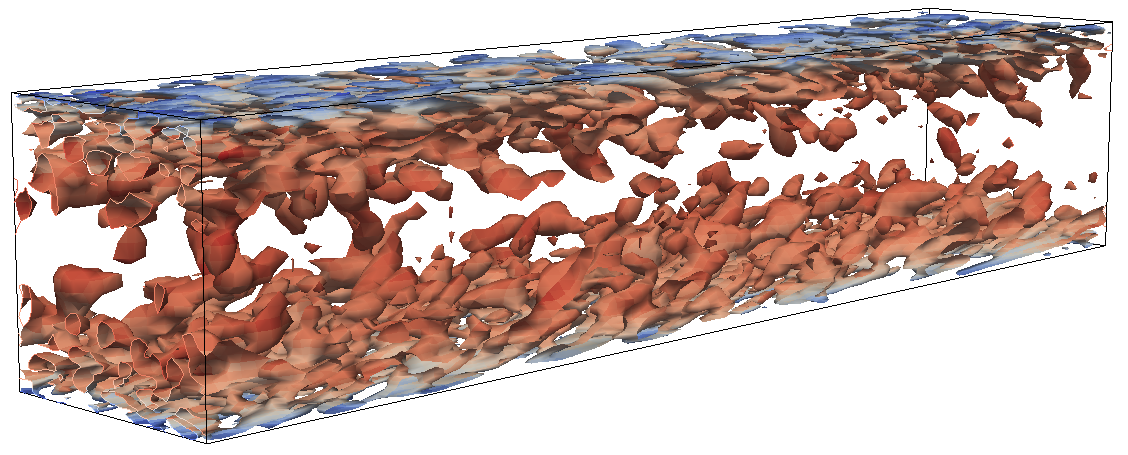
\includegraphics[width=\linewidth]{TInF-NE-04.png} \label{SEMlambda}
        \caption{the turbulentSEMInlet boundary condition}
     \end{subfigure}
    \begin{subfigure}[b]{0.6\linewidth}
        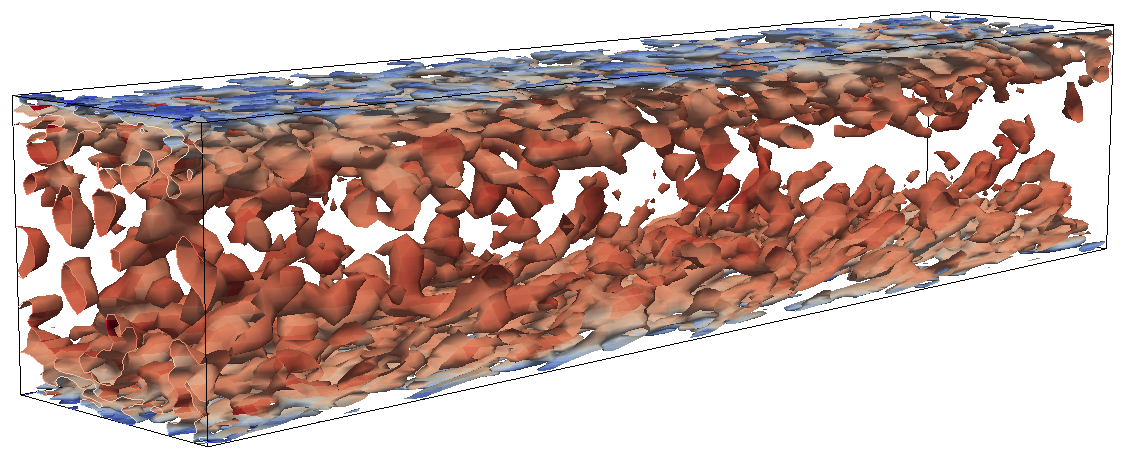
\includegraphics[width=\linewidth]{TInF-NE-05.png}
        \caption{the turbulentDFMInlet boundary condition} \label{DFMlambda}
    \end{subfigure}
     \begin{subfigure}[b]{0.6\linewidth}
        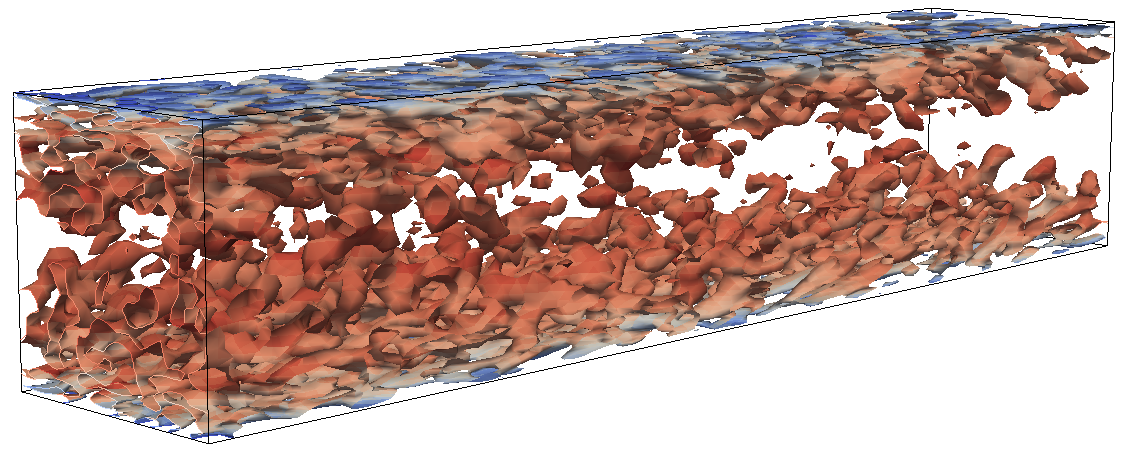
\includegraphics[width=\linewidth]{TInF-NE-06.png}
        \caption{the turbulentATSMInlet (type R) boundary condition} \label{ATSMRlambda}
    \end{subfigure}
    \begin{subfigure}[b]{0.6\linewidth}
        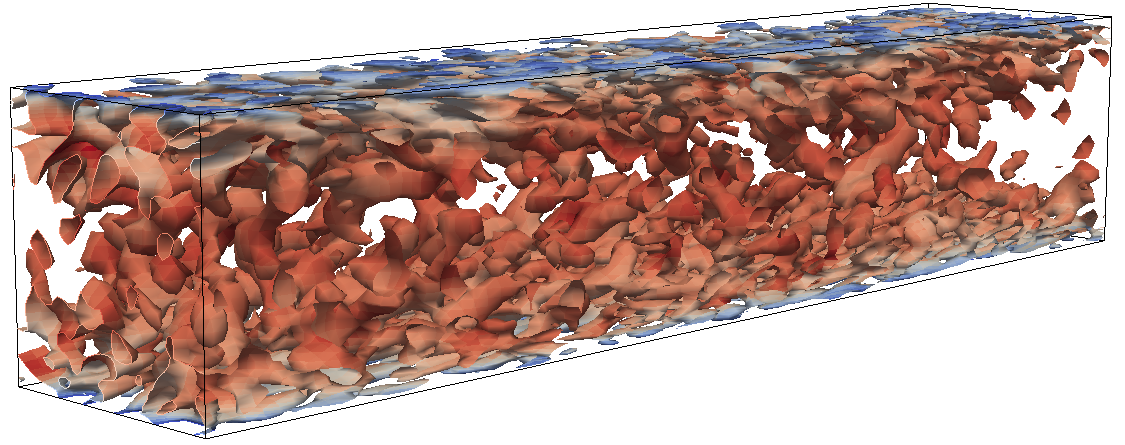
\includegraphics[width=\linewidth]{TInF-NE-07.png}
        \caption{the turbulentATSMInlet (type L) boundary condition} \label{ATSMLlambda}
    \end{subfigure}
      \caption{Visualization of turbulent vortices in channel flow simulations by contour-surfaces of $\lambda_2 = 50$} \label{lambda2}
\end{figure}

\begin{figure}[H]
\centering
    \begin{subfigure}[b]{0.7\linewidth}
        \includegraphics[width=\linewidth]{TInF-NE-08.eps}
        \caption{the turbulentSEMInlet boundary condition}
     \end{subfigure}
     \begin{subfigure}[b]{0.7\linewidth}
        \includegraphics[width=\linewidth]{TInF-NE-09.eps}
        \caption{the turbulentDFSEMInlet boundary condition}
    \end{subfigure}
    \begin{subfigure}[b]{0.7\linewidth}
        \includegraphics[width=\linewidth]{TInF-NE-10.eps}
        \caption{the turbulentATSMInlet (type R) boundary condition}
    \end{subfigure}
    \begin{subfigure}[b]{0.7\linewidth}
        \includegraphics[width=\linewidth]{TInF-NE-11.eps}
        \caption{the turbulentATSMInlet (type L) boundary condition}
    \end{subfigure}
      \caption{Inflow channel simulations: comparison of pressure fluctuations vs. axial distance for different synthetic methods at $\mathrm{Re}_{\tau} = 395$}\label{pressure}
\end{figure}

\begin{figure}[H]
\centering
\includegraphics[width=\linewidth]{TInF-NE-12.eps}
\caption{Main components of the Reynolds stress tensor at different sections in the channel flow simulation with DFM}\label{dfm}
 \end{figure}
 
 
\begin{figure}[H]
\centering
\includegraphics[width=\linewidth]{TInF-NE-13.eps}
\caption{Main components of the Reynolds stress tensor at different sections in the channel flow simulation with SEM}\label{sem}
 \end{figure}


\begin{figure}[H]
\centering
\includegraphics[width=\linewidth]{TInF-NE-14.eps}
\caption{Main components of the Reynolds stress tensor at different sections in the channel flow simulation with ATSM-R}\label{atsmr}
 \end{figure}
 
 
\begin{figure}[H]
\centering
\includegraphics[width=\linewidth]{TInF-NE-15.eps}
\caption{Main components of the Reynolds stress tensor at different sections in the channel flow simulation with ATSM-L}\label{atsml}
 \end{figure}

% \appendix
% \chapter{More Monticello Candidates}

\pagestyle{plain}
{
  \renewcommand{\thispagestyle}[1]{}
  \printbibliography           
}

\end{document}
